\documentclass[../../main]{subfiles}
\pagestyle{fancy}

\begin{document}

\chapter{The External CMI}
\thispagestyle{fancy}

\todo[inline]{Introduction.}

\section{$\hod$ mice}
\todo[inline]{Provide overview of this section.}

\subsection{Iteration strategies}

\todo[inline]{At some point we should mention that we adopt John`s
  convention of hiding the degree of iteration trees, always taking
  the maximal possible degree. And that all of our trees are (stacks
  of) normal trees.}

\defi{ Let $\vec{\mathcal{T}}$ be a
  stack of normal trees. We write $\lh(\vec{\mathcal{T}})$ for the
  length of $\vec{\mathcal{T}}$ and $\mathcal{T}_{\alpha}$ for the
  $\alpha$th tree in $\vec{\mathcal{T}}$, so that
  \[
    \vec{\mathcal{T}} = (\mathcal{T}_{\alpha} \mid \alpha <
    \lh(\vec{\mathcal{T}})).
  \]
  For $\alpha < \beta < \lh(\vec{\mathcal{T}})$,
  $\gamma < \lh(\mathcal{T}_{\alpha})$,
  $\eta < \lh(\mathcal{T}_{\beta})$ we let
  $\mathcal{M}^{\mathcal{T}_{\alpha}}_{\gamma}$ be the model with
  index $\gamma$ in the tree $\mathcal{T}_{\alpha}$ and write
  \[
    \pi^{\vec{\mathcal{T}}}_{(\alpha, \gamma), (\beta, \eta)} \colon
    \mathcal{M}^{\mathcal{T}_{\alpha}}_{\gamma} \to
    \mathcal{M}^{\mathcal{T}_{\beta}}_{\eta}
  \]
  for the corresponding embedding, provided it exists. \\
  We also write
  \[
    \pi^{\vec{\mathcal{T}}}_{\alpha, \beta} \colon
    \mathcal{M}^{\mathcal{T}_{\alpha}}_{0} \to
    \mathcal{M}^{\mathcal{T}_{\beta}}_{0}.
  \]
  If $\vec{\mathcal{T}}$ has a last model, i.e. if
  $\lh(\vec{\mathcal{T}}) = \xi + 1$ and
  $\mathcal{M}^{\mathcal{T}_{\xi}}_{\infty}$ exists, we let
  $\mathcal{M}^{\vec{\mathcal{T}}}_{\infty} :=
  \mathcal{M}^{\mathcal{T}_{\xi}}_{\infty}$ and
  $\pi^{\vec{\mathcal{T}}} \colon \mathcal{M}^{\mathcal{T}_{0}}_{0}
  \to \mathcal{M}^{\vec{\mathcal{T}}}_{\infty}$ be the associated
  embedding.  }


\defi{ Let $\Sigma$ be an iteration strategy and
  $(\vec{\mathcal{T}}, N) \in I(\mathcal{M}_{\Sigma}, \Sigma)$. We
  write $\Sigma_{\vec{\mathcal{T}}, N}$
  \index{$\Sigma_{\vec{\mathcal{T}}, N}$} for the iteration strategy
  on $N$ given by
  \[
    \Sigma_{\vec{\mathcal{T}}, N}(\vec{\mathcal{U}}) :=
    \Sigma(\vec{\mathcal{T}} ^{\frown} \vec{\mathcal{U}}).
  \]
  We call $\Sigma_{\vec{\mathcal{T}}, N}$ the
  \textbf{$(\vec{\mathcal{T}}, N)$-tail strategy}of $\Sigma$.
  \index{$(\vec{\mathcal{T}}, N)$-tail strategy}}

\defi{ \todo[inline]{at the very end we should remove those definitions that we didn`t need}
  Let $\Sigma$ be an iteration strategy.
  \begin{enumerate}
  \item $\Sigma$ has the \textbf{Dodd-Jensen property} \index{$\Sigma$
      has the Dodd-Jensen property} if for all
    $(\vec{\mathcal{T}}, N) \in I(\mathcal{M}_{\Sigma}, \Sigma)$ and
    all $\pi \colon \mathcal{M}_{\Sigma} \to_{\Sigma_{1}} N$ we have
    $\pi^{\vec{\mathcal{T}}}(\alpha) \le \pi(\alpha)$ for all
      $\alpha \in o(\mathcal{M}_{\Sigma})$.
    \item $\Sigma$ has the \textbf{positional Dodd-Jensen property}
      \index{$\Sigma$ has the positional Dodd-Jensen property} if
      $\Sigma_{\vec{\mathcal{T}},N}$ has the Dodd-Jensen property for
      all $(\vec{\mathcal{T}},N) \in I(\mathcal{M}_{\Sigma}, \Sigma)$.
    \item $\Sigma$ is \textbf{weakly positional} \index{$\Sigma$ is
        weakly positional} if
      $\Sigma_{\vec{\mathcal{T}},N} = \Sigma_{\vec{\mathcal{U}},N}$
      for all
      $(\vec{\mathcal{T}},N), (\vec{\mathcal{U}}, N) \in
      I(\mathcal{M}_{\Sigma}, \Sigma)$.
    \item $\Sigma$ is \textbf{positional} \index{$\Sigma$ is positional}
      if $\Sigma_{\vec{\mathcal{T}}, N}$ is weakly positional for all
      $(\vec{\mathcal{T}}, N) \in I(\mathcal{M}_{\Sigma}, \Sigma)$.
    \item $\Sigma$ is \textbf{weakly commuting} \index{$\Sigma$ is
        weakly commuting} if
      $\pi^{\vec{\mathcal{T}}} = \pi^{\vec{\mathcal{U}}}$ for all
      $(\vec{\mathcal{T}}, N), (\vec{\mathcal{U}}, N) \in
      I(\mathcal{M}_{\Sigma}, \Sigma)$.
    \item $\Sigma$ is \textbf{commuting} \index{$\Sigma$ is commuting}
      if $\Sigma_{\vec{\mathcal{T}}, N}$ is weakly commuting for all
      $(\vec{\mathcal{T}}, N) \in I(\mathcal{M}_{\Sigma}, \Sigma)$.
    \item $\Sigma$ is \textbf{weakly pullback consistent}
      \index{$\Sigma$ is weakly pullback consistent} if
      $\Sigma^{\vec{\mathcal{T}}} = \Sigma$ for all
      $(\vec{\mathcal{T}}, N) \in I(\mathcal{M}_{\Sigma}, \Sigma)$.
    \item $\Sigma$ is \textbf{pullback consistent} \index{$\Sigma$ is
        pullback consistent} if $\Sigma_{N, \vec{\mathcal{T}}}$ is
      weakly pullback consistent for all
      $(\vec{\mathcal{T}}, N) \in I(\mathcal{M}_{\Sigma}, \Sigma)$.      
  \end{enumerate}
}

\defi{

  If $\Sigma$ is positional, $\Sigma_{\vec{\mathcal{T}}, N}$ doesn`t
  depend on $\vec{\mathcal{T}}$ and hence we simply write $\Sigma_{N}$
  \index{$\Sigma_{N}$} for this tail strategy.

}

\defi{ An iteration strategy $\Sigma$ has \textbf{branch condensation}
  (see \autoref{fig:branch condensation}) \index{Branch condensation} if
  for any two stacks $\vec{\mathcal{T}}, \vec{\mathcal{U}}$ on
  $\mathcal{M}_{\Sigma}$ such that
  \begin{enumerate}
  \item $\vec{\mathcal{T}}, \vec{\mathcal{U}}$ are according to $\Sigma$,
  \item $\vec{\mathcal{U}}$ is a stack of successor length
    $\gamma + 1$ and $\vec{\mathcal{U}}$`s last component
    $\mathcal{U}_{\gamma}$is of limit length,
  \item $\vec{\mathcal{T}}$ has a last model $N$ such that
    $(\vec{\mathcal{T}}, N) \in I(\mathcal{M}_{\Sigma}, \Sigma)$,
  \item there is some branch $c$ such that
    $\pi^{\vec{\mathcal{U}}}_{c}$ exists and for some
    $\pi \colon \mathcal{M}^{\vec{\mathcal{U}}}_{c} \to_{\Sigma_{1}}
    N$ we have
    \[
      \pi^{\vec{\mathcal{T}}} = \pi \circ \pi^{\vec{\mathcal{U}}}_{c}.
    \]
  \end{enumerate}
  Then $c = \Sigma(\vec{\mathcal{U}})$.
}

\begin{figure}
  \centering
  \begin{tikzcd}[row sep=large, column sep=large]
    & & N \\
    \mathcal{M}_{\Sigma} \arrow[urr, "\pi^{\vec{\mathcal{T}}}"] \arrow[drr, "\pi^{\vec{\mathcal{U}}}_{c}"]& & \\
    & & \mathcal{M}^{\vec{\mathcal{U}}}_{c} \arrow[uu, "\pi"]
    \end{tikzcd}
  \caption{Branch condensation}
  \label{fig:branch condensation}
\end{figure}

  \defi{
    % Caution:
    % $(\mathcal{M}, \mathcal{T}), (\mathcal{N}, \mathcal{U})$ are
    % flipped when compared to Grigor`s thesis
    Let $\mathcal{M}, \mathcal{N}$ be layered hybrid premice and
    $\mathcal{T}, \mathcal{U}$ be normal trees on
    $\mathcal{M}, \mathcal{N}$ respectively.
    \textbf{$(\mathcal{M}, \mathcal{T})$ is a hull of
      $(\mathcal{N}, \mathcal{U})$} \index{Hull of a normal tree} if
    there are
    \begin{enumerate}
    \item an embedding, $\pi \colon \mathcal{M} \to_{\Sigma_{1}} \mathcal{N}$ and
    \item an order-preserving map
      $\sigma \colon \lh(\mathcal{T}) \to \lh(\mathcal{U})$
    \end{enumerate}
    such that
    \begin{enumerate}
    \item $\alpha \le_{\mathcal{T}} \beta \iff \sigma(\alpha) \le_{\mathcal{U}} \sigma(\beta)$
    \item
      $[\alpha,\beta]_{\mathcal{T}} \cap \mathcal{D}^{\mathcal{T}} =
      \emptyset \iff [\sigma(\alpha),\sigma(\beta)]_{\mathcal{U}} \cap
      \mathcal{D}^{\mathcal{U}} = \emptyset$,
    \item
      $\pi_{\alpha} \colon \mathcal{M}_{\alpha}^{\mathcal{T}} \to
      \mathcal{M}_{\sigma(\alpha)}^{\mathcal{U}}$ and
      $\pi_{\alpha}(E^{\mathcal{T}}_{\alpha}) =
      E^{\mathcal{U}}_{\sigma(\alpha)}$,
    \item for $\beta < \alpha$ we have
      $\pi_{\alpha} \restriction \lh(E_{\beta}^{\mathcal{T}}) + 1 =
      \pi_{\beta} \restriction \lh(E_{\beta}^{\mathcal{T}}) + 1$,
    \item for $\alpha \le_{\mathcal{T}} \beta$ with
      $[\alpha,\beta]_{\mathcal{T}} \cap \mathcal{D}^{\mathcal{T}}$ we
      have
      $\pi_{\beta} \circ \pi^{\mathcal{T}}_{\alpha,\beta} =
      \pi^{\mathcal{U}}_{\sigma(\alpha), \sigma(\beta)} \circ
      \pi_{\alpha}$,
      \item if $\beta = \pred_{\mathcal{T}}(\alpha + 1)$, then
      $\sigma(\beta) = \pred_{\mathcal{U}}(\sigma(\alpha + 1))$ and
      $\pi_{\alpha+1}([a,f]_{E^{\mathcal{T}}_{\alpha}}) =
      [\pi_{\alpha}(a),
      \pi_{\beta}(f)]_{E^{\mathcal{T}}_{\sigma(\alpha)}}$ and
    \item $0 \le_{\mathcal{U}} \sigma(0)$,
      $[0, \sigma(0)] \cap \mathcal{D}^{\mathcal{U}} = \emptyset$ and
      $\pi_{0} = \pi^{\mathcal{U}}_{0, \sigma(0)} \circ \pi$,
    \end{enumerate}
    (See \autoref{fig:hull of U})
  }

  \defi{ Let $\mathcal{M}, \mathcal{N}$ be layered hybrid premice and
    $\vec{\mathcal{T}}, \vec{\mathcal{U}}$ be stacks of normal trees
    on $\mathcal{M}, \mathcal{N}$ respectively.
    \textbf{$(\mathcal{M}, \vec{\mathcal{T}})$ is a hull of
      $(\mathcal{N}, \vec{\mathcal{U}})$} \label{hull of a stack of
      normal trees} if there are
    
  \begin{enumerate}
  \item an order presercing map $\sigma \colon \lh(\vec{\mathcal{T}}) \to \lh(\vec{\mathcal{U}})$,
  \item a sequence $(\sigma_{\alpha} \mid \alpha < \lh(\vec{\mathcal{T}}))$ of order preserving maps $\sigma_{\alpha} \colon \lh(\mathcal{T}_{\alpha}) \to \lh(\mathcal{U}_{\sigma(\alpha)})$,
  \item
    $(\pi_{\alpha,\beta} \mid \alpha < \lh(\vec{\mathcal{T}}) \wedge
    \beta < \lh(\mathcal{T}_{\alpha}))$ such that
    \begin{enumerate}
    \item $\pi_{0,0} = \pi^{\vec{\mathcal{U}}}_{0, \sigma(0)}$ (so
      that $\pi_{0,0} = \id$ if $\sigma(0) = 0$),
    \item for $\alpha < \lh(\vec{\mathcal{T}})$
      \[
	\pi_{\alpha,0} \colon \mathcal{M}_{\alpha}^{\vec{\mathcal{T}}} \to_{\Sigma_{1}} \mathcal{M}^{\vec{\mathcal{U}}}_{\sigma(\alpha)}
      \]
      and
      $(\mathcal{M}^{\vec{\mathcal{T}}}_{\alpha},
      \mathcal{T}_{\alpha})$ is a $(\pi_{\alpha,0}, \sigma_{0})$-hull
      of
      $(\mathcal{M}^{\vec{\mathcal{U}}}_{\sigma(\alpha)},
      \mathcal{U}_{\sigma(\alpha)})$,
    \item $\alpha < \beta < \lh(\vec{\mathcal{T}})$ and
      $\pi^{\vec{\mathcal{T}}}_{(\alpha,\gamma), (\beta, \eta)}$
      exists, then
      $\pi^{\vec{\mathcal{U}}}_{(\sigma(\alpha),
        \sigma_{\alpha}(\gamma)), (\sigma(\beta),
        \sigma_{\beta}(\eta))}$ exists and
      \[
	\pi_{\beta,\eta} \circ
        \pi^{\vec{\mathcal{T}}}_{(\alpha,\gamma), (\beta,\eta)} =
        \pi^{\vec{\mathcal{U}}}_{(\sigma(\alpha),
          \sigma_{\alpha}(\gamma)), (\sigma(\beta),
          \sigma_{\beta}(\eta))} \circ \pi_{\alpha, \gamma}.
      \]
    \end{enumerate}
  \end{enumerate}
  (See \autoref{fig:hull of stack of normal tree})
}

\begin{figure}
  \centering
  % 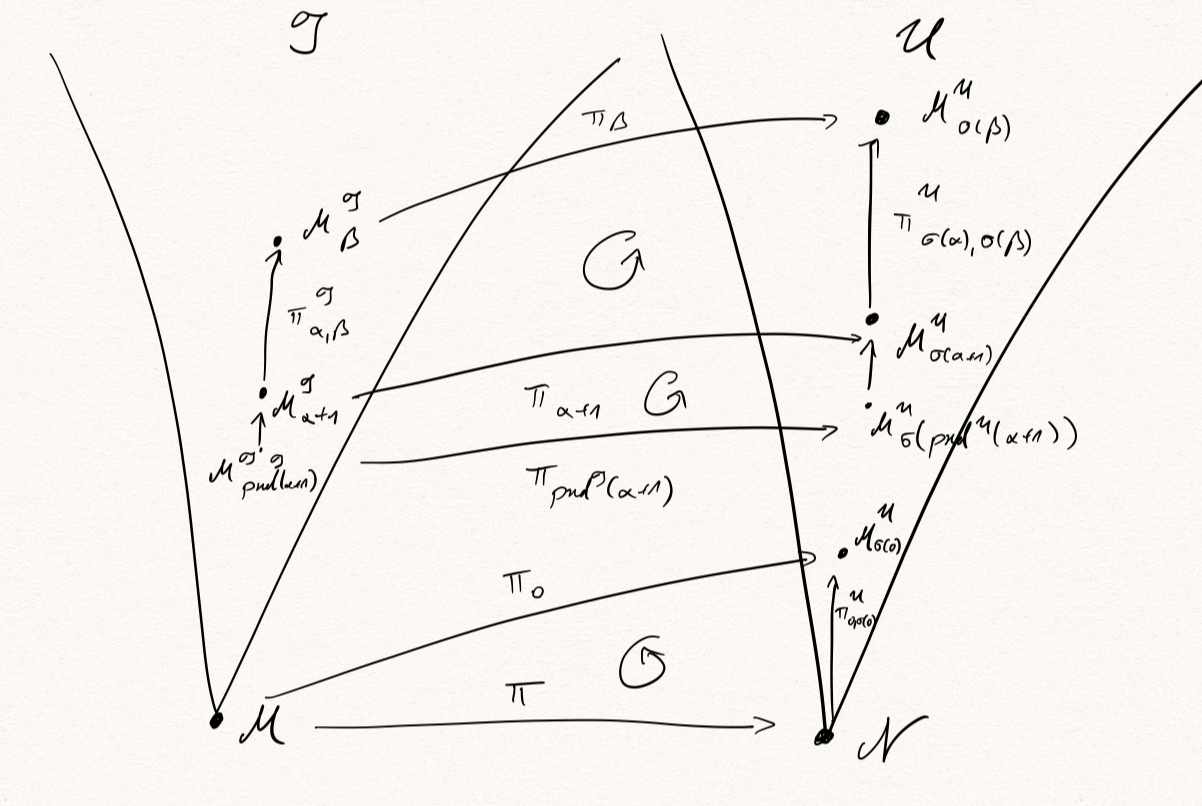
\includegraphics[width=300px]{\string~/gitsky/phd/gfx/hull-of-U.png}
    \begin{tikzpicture}
  \coordinate (rootl) at (0,0);
  \coordinate (rootr) at (7,0);
  
  \coordinate (treel) at (-2,7);
  \coordinate (treer) at (2,7);

  \coordinate (modelroot) at (0,0);
  \coordinate (modelroottarget) at (0,1.5);
  \coordinate (model0) at (0,2.5);
  \coordinate (model1) at (0,4);
  \coordinate (model2) at (0,6);
  \coordinate (offsetr) at (0,1);

  \draw [dotted] (rootl) -- ($(rootl) + (treel)$);
  \draw [dotted] (rootl) -- ($(rootl) + (treer)$);

  \draw [dotted] (rootr) -- ($(rootr) + (treel) + (offsetr)$);
  \draw [dotted] (rootr) -- ($(rootr) + (treer) + (offsetr)$);

  % models of left tree
  \fill ($(rootl) + (modelroot)$) circle[radius=1pt] node[left]
  {$\mathcal{M}^{\mathcal{T}}_{0}$};
  \fill ($(rootl) + (model0)$) circle[radius=1pt] node[left]
  {$\mathcal{M}^{\mathcal{T}}_{\pred^{\mathcal{T}}(\alpha+1)}$};
  \fill ($(rootl) + (model1)$) circle[radius=1pt] node[left]
  {$\mathcal{M}^{\mathcal{T}}_{\alpha+1}$};
  \fill ($(rootl) + (model2)$) circle[radius=1pt] node[left]
  {$\mathcal{M}^{\mathcal{T}}_{\beta}$};

  % models of right tree
  \fill ($(rootr) + (modelroot)$) circle[radius=1pt] node[right]
  {$\mathcal{M}^{\mathcal{U}}_{0}$};
  \fill ($(rootr) + (modelroottarget)$) circle[radius=1pt] node[right]
  {$\mathcal{M}^{\mathcal{U}}_{\sigma(0)}$};
  \fill ($(rootr) + (model0) + (offsetr)$) circle[radius=1pt] node[right]
  {$\mathcal{M}^{\mathcal{U}}_{\sigma(\pred^{\mathcal{T}}(\alpha+1))}$};
  \fill ($(rootr) + (model1) + (offsetr)$) circle[radius=1pt] node[right]
  {$\mathcal{M}^{\mathcal{U}}_{\sigma(\alpha+1)}$};
  \fill ($(rootr) + (model2) + (offsetr)$) circle[radius=1pt] node[right]
  {$\mathcal{M}^{\mathcal{U}}_{\sigma(\beta)}$};

  % embeddings between trees
  \draw [->] ($(rootl) + (modelroot)$) -- node[below]{$\pi$}($(rootr) + (modelroot)$);
  \draw [->] ($(rootl) + (modelroot)$) -- node[above]{$\pi_{0}$}($(rootr) + (modelroottarget)$);
  \draw [->] ($(rootr) + (modelroot)$) -- node[right]{$\pi^{\mathcal{U}}_{0, \sigma(0)}$} ($(rootr) + (modelroottarget)$);

  \draw [->] ($(rootl) + (model0)$) -- node[below]{$\pi_{\pred^{\mathcal{T}}(\alpha+1)}$} ($(rootr) + (model0) + (offsetr)$);
  \draw [->] ($(rootl) + (model1)$) -- node[below]{$\pi_{\alpha+1}$} ($(rootr) + (model1) + (offsetr)$);
  \draw [->] ($(rootl) + (model2)$) -- node[below]{$\pi_{\beta}$} ($(rootr) + (model2) + (offsetr)$);

  % embeddings in left tree
  \draw [->] ($(rootl) + (model0)$) -- node[right]{$\pi^{\mathcal{T}}_{\pred^{\mathcal{T}}(\alpha+1), \alpha+1}$}($(rootl) + (model1)$);
  \draw [->] ($(rootl) + (model1)$) -- node[right]{$\pi^{\mathcal{T}}_{\alpha+1, \beta}$}($(rootl) + (model2)$);

  % embeddings in right tree
  \draw [->] ($(rootr) + (model0) + (offsetr)$) -- node[right]{$\pi^{\mathcal{U}}_{\sigma(\pred^{\mathcal{T}}(\alpha+1)), \sigma(\alpha+1)}$}($(rootr) + (model1) + (offsetr)$);
  \draw [->] ($(rootr) + (model1) + (offsetr)$) -- node[right]{$\pi^{\mathcal{U}}_{\sigma(\alpha+1), \sigma(\beta)}$}($(rootr) + (model2) + (offsetr)$);
\end{tikzpicture}
  \caption{$\mathcal{T}$ is a hull of $\mathcal{U}$}
  \label{fig:hull of U}

\end{figure}

\begin{figure}
  \centering
  % placeholder
  % 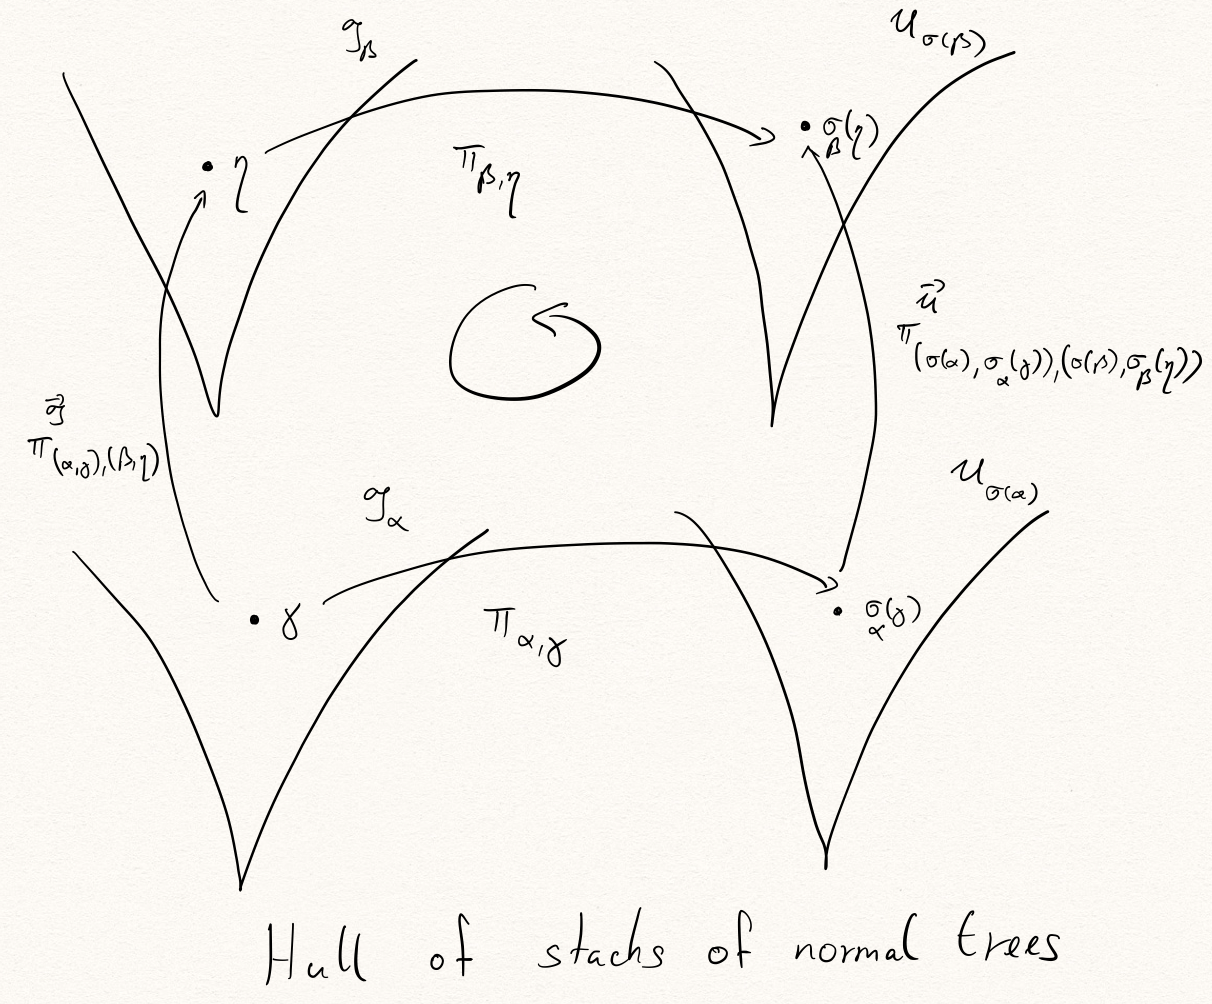
\includegraphics[width=300px]{\string~/gitsky/phd/gfx/hull-of-vec-U.png}

  \begin{tikzpicture}
  \coordinate (rootul) at (0,0);
  \coordinate (rootur) at (5,1);
  \coordinate (rootdl) at (0,-4);
  \coordinate (rootdr) at (5,-3);
  
  \coordinate (treel) at (-2,3);
  \coordinate (treer) at (2,3);
  \coordinate (model) at (0,2);

  % Tree upper left
  \draw (rootul) node[below]{$\mathcal{T}_{\beta}$} --
  ($(rootul) + (treel)$);
  \draw (rootul) -- ($(rootul) + (treer)$);
  \fill ($(rootul) + (model)$) circle[radius=1pt] node[below right]
  {$\mathcal{M}^{\mathcal{T}_{\beta}}_{\eta}$};

  % Tree upper right
  \draw (rootur) node[below]{$\mathcal{U}_{\sigma(\beta)}$} --
  ($(rootur) + (treel)$);
  \draw (rootur) -- ($(rootur) + (treer)$);
  \fill ($(rootur) + (model)$) circle[radius=1pt] node[right]
  {$\mathcal{M}^{U_{\sigma(\beta)}}_{\sigma_{\beta}(\eta)}$};

  % Tree down left
  \draw (rootdl) node[below]{$\mathcal{T}_{\alpha}$} --
  ($(rootdl) + (treel)$);
  \draw (rootdl) -- ($(rootdl) + (treer)$);
  \fill ($(rootdl) + (model)$) circle[radius=1pt] node[below right]
  {$\mathcal{M}^{T_{\alpha}}_{\gamma}$};

  % Tree down right
  \draw (rootdr) node[below]{$\mathcal{U}_{\sigma(\alpha)}$} --
  ($(rootdr) + (treel)$);
  \draw (rootdr) -- ($(rootdr) + (treer)$);
  \fill ($(rootdr) + (model)$) circle[radius=1pt] node[right]
  {$\mathcal{M}^{U_{\sigma(\alpha)}}_{\sigma_{\alpha}(\gamma)}$};

  % Embedding left
  \draw [->] ($(rootdl) + (model)$) to [out=135,in=225]
  node[left]{$\pi^{\vec{\mathcal{T}}}_{(\alpha,\gamma),(\beta,\eta)}$}
  ($(rootul) + (model)$);

  % Embedding right
  \draw [->] ($(rootdr) + (model)$) to [out=45,in=315]
  node[right]{$\pi^{\vec{\mathcal{U}}}_{(\sigma(\alpha),
      \sigma_{\alpha}(\gamma)), (\sigma(\beta),
      \sigma_{\beta}(\eta))}$}($(rootur) + (model)$);

  % Embedding up
  \draw [->] ($(rootul) + (model)$) to node[above]{$\pi_{\beta,\eta}$}
  ($(rootur) + (model)$);

  % Embedding down
  \draw [->] ($(rootdl) + (model)$) to
  node[above]{$\pi_{\alpha,\gamma}$} ($(rootdr) + (model)$);
\end{tikzpicture}
  \caption{$\vec{\mathcal{T}}$ is a hull of $\vec{\mathcal{U}}$}
  \label{fig:hull of stack of normal tree}
\end{figure}

\defi{ Let $\mathcal{M}$ be a layered hybrid premouse and $\Sigma$ be
  a (partial) iteration strategy for $\mathcal{M}$. $\Sigma$ has
  \textbf{hull condensation} \index{$\Sigma$ has hull condensation} if
  the follwing holds true for any two stacks
  $\vec{\mathcal{T}}, \vec{\mathcal{U}}$ on
  $\mathcal{M}$. \\
  If $\vec{\mathcal{U}}$ is according to $\Sigma$ and
  $\vec{\mathcal{T}}$ is a hull of $\vec{\mathcal{U}}$, then
  $\vec{\mathcal{T}}$ is according to $\Sigma$.  }

\lemm{ Let $\Sigma$ be an iteration strategy. Then the following hold
  true.
  \begin{enumerate}
  \item If $\Sigma$ has hull condensation then it is pullback consistent.
  \item If $\Sigma$ is positional and pullback consistent then it is commuting.
  \end{enumerate}
}

\proof{
  See \cite[Proposition~2.36]{sargsyan2015hod}.
}

\subsection{Layered Hybrid Mice}

\todo[inline]{Define strategy mice as a particular kind of hybrid
  mice, hod mice/pairs and put in positional and commuting in the
  definition, state comparison. Introduce derived models of hod mice
  and how they relate to the Solovay hierarchy.\\
  Define $\Sigma$-mouse}

\defi{ Let $\mathcal{M}$ be a transitive set (or structure). We let
  $o(\mathcal{M}) := \mathcal{M} \cap \on$ \index{$o(\mathcal{M})$} be
  the ordinal height of $\mathcal{M}$.  }

\defi{ Let $\mathcal{M}$ be a (hybrid) premouse and $\alpha \le o(\mathcal{M})$. We let
  \begin{enumerate}
  \item $\mathcal{M} || \alpha$ \index{$\mathcal{M}\|\|\alpha$} be the
    initial segment of $\mathcal{M}$ of height $\alpha$ including its
    top extender and
  \item $\mathcal{M} | \alpha$ \index{$\mathcal{M}\|\alpha$} be the
    passive initial segment of $\mathcal{M}$ of height $\alpha$,
    i.e. $\mathcal{M} || \alpha$ but without the top extender.
  \end{enumerate}
}

\defi{ Let $\mathcal{M}$ be a $\mathcal{J}$-structure \footnote{See
    \cite{zeman2011inner} for the basics on $\mathcal{J}$-structures,
    premice and their fine structure.} and
  $\alpha \le o(\mathcal{M})$. We write
  $\mathcal{J}^{\mathcal{M}}_{\alpha}$ for the $\alpha$th level of
  $\mathcal{M}$`s construction. }

\defi{ A \textbf{potential layered hybrid premouse} (over $X$)
  \index{potential layered hybrid premouse} is an acceptable
  $\mathcal{J}$-structure of the form
  $\mathcal{M} = (J^{\vec{E},f}_{\alpha}(X); \in, \vec{E}, B, f)$ $X$
  such that
  \begin{enumerate}
  \item $\vec{E}$ is a fine extender sequence (over $X$),
  \item $f$ is a function with domain
    $Y \subseteq \alpha$ such that $f(\gamma)$, for each
    $\gamma \in Y$, is a shift of an amenable function
    that typically codes part of an iteration strategy for
    $\mathcal{M}$,
  \end{enumerate}
  We will often write
  $\vec{E}^{\mathcal{M}}, f^{\mathcal{M}}, Y^{\mathcal{M}}$ for
  $\vec{E},f,Y$ as above. \\
  If all proper initial segments of $\mathcal{M}$ are sound, we say
  that $\mathcal{M}$ is a \textbf{layered hybrid premouse}.
  \index{layered hybrid premouse}. }

In our case, assuming $X$ is a self-well-ordered set,
$Y^{\mathcal{M}}$ is determined by the \textbf{standard indexing scheme}
(see \cite[Definition~1.18]{sargsyan2015hod}).

%%%%%%%%%%%%%%%%%% 
For more details, see \cite{sargsyan2015hod}.
%%%%%%%%%%%%%%%%%%

\defi{ Let $\Sigma$ be a strategy for a layered hybrid premouse
  $\mathcal{M}$. For $\alpha \le o(M)$ we let
  $\Sigma_{\mathcal{M} | \alpha}$ be the $\id$-pullback iteration
  strategy on $\mathcal{M} | \alpha$ induced by $\Sigma$, i.e. a stack
  $\vec{\mathcal{T}}$ on $\mathcal{M} | \alpha$ is according to
  $\Sigma_{\mathcal{M} | \alpha}$ iff $\id \vec{\mathcal{T}}$ on
  $\mathcal{M}$, given by the copy construction via $\id$ (see
  \cite[4.1]{steel2010outline}), is according to $\Sigma$.}

\defi{ A \textbf{layered strategy premouse} \index{layered strategy
    premouse} $\mathcal{M}$ is a layered hybrid premouse such that
  \begin{enumerate}
  \item $f^{\mathcal{M}}(\gamma)$ codes a partial iteration strategy
    $\Sigma^{\mathcal{M}}_{\gamma}$ for $\mathcal{M} | \gamma$ and
  \item For $\gamma_{0}, \gamma_{1} \in Y^{\mathcal{M}}$, if
    $\gamma_{0} < \gamma_{1}$ then
    $(\Sigma^{\mathcal{M}}_{\gamma_{1}})_{\mathcal{M} | \gamma_{0}}
    \subseteq \Sigma^{\mathcal{M}}_{\gamma_{0}}$.    
  \end{enumerate}
  We also write $\Sigma^{\mathcal{M}}$ for the the strategy coded by
  $f^{\mathcal{M}}$.
}

\defi{
  Let $\mathcal{M}$ be a layered strategy premouse and $\Sigma$
  be an iteration strategy for $\mathcal{M}$. $\mathcal{M}$ is a
  \textbf{$\Sigma$-premouse} \index{$\Sigma$-premouse} if
  $\Sigma^{\mathcal{M}} \subseteq \Sigma$.
}

\begin{definition}
  \index{$I(\mathcal{M}_{\Sigma}, \Sigma)$}
  \index{$pI(\mathcal{M}_{\Sigma}, \Sigma)$}
  Let $\Sigma$ be an iteration strategy. We write
  $\mathcal{M}_{\Sigma}$ \index{$\mathcal{M}_{\Sigma}$} for the
  (layered hybrid) premouse $\mathcal{N}$ such that $\Sigma$ is an
  iteration strategy for $\mathcal{N}$.  We also let
  \eq{
    I(\mathcal{M}_{\Sigma}, \Sigma) := \{ (\vec{\mathcal{T}}, N) \mid \ & \vec{\mathcal{T}} \text{ is a stack of normal trees on } \mathcal{M}_{\Sigma} \text{ according to } \Sigma \text{,} \\
    & \pi^{\vec{\mathcal{T}}} \text{ exist and $N$ is the last model of } \vec{\mathcal{T}} \}.
  }

  and
  \eq{
    pI(\mathcal{M}_{\Sigma}, \Sigma) :=
    \{ N \mid \exists \vec{\mathcal{T}} \colon (\vec{\mathcal{T}}, N) \in I(\mathcal{M}_{\Sigma}, \Sigma) \}.\tag*{$\dashv$}
  }
\end{definition}

\defi{ A $\Sigma$-premouse $\mathcal{M}$ is a \textbf{$\Sigma$-mouse}
  \index{$\Sigma$-mouse} if there is a $\omega_{1}+1$-iteration
  strategy $\Lambda$ such that all
  $\mathcal{N} \in pI(\mathcal{M}, \Lambda)$, $\mathcal{N}$ are
  themselves $\Sigma$-premice.
}

\defi{ Let $a$ be a transitive self-well-ordered set and let $\Sigma$
  be an iteration strategy with hull-condensation such that
  $\mathcal{M}_{\Sigma} \in a$ and let $\Gamma$ be a pointclass which
  is closed under Boolean operations and continuous images and
  preimages. Define the $(\Gamma, \Sigma)$-$\lp$ stack over $a$
  \index{Lp$^{\Gamma, \Sigma}$} recursively as follows:

  \begin{enumerate}
  \item $\lp^{\Gamma, \Sigma}_{0}(a) := a \cup \{ a \}$,
  \item
    $\lp^{\Gamma, \Sigma}_{\alpha + 1}(a) := \bigcup \{ \mathcal{M}
    \mid \mathcal{M} \text{ is a sound } \Sigma \text{-mouse over }
    \lp^{\Gamma, \Sigma}_{\alpha}(a) \\ \text{ projecting to }
    o(\lp^{\Gamma, \Sigma}_{\alpha}(a)) \text{ and having an iteration
      strategy in } \Gamma \}$,
  \item
    $\lp^{\Gamma, \Sigma}_{\lambda}(a) := \bigcup_{\alpha < \lambda}
    \lp^{\Gamma, \Sigma}(a)$ for limit $\lambda$.
  \end{enumerate}
  We also let
  $\lp^{\Gamma, \Sigma}(a) := \lp^{\Gamma, \Sigma}_{1}(a)$.  }

\subsection{$\hod$ Mice}

\defi[][defi:hod premouse]{Suppose
  $\mathcal{P} = (J^{\vec{E},f}(X); \in, \vec{E}, f, B)$ is a layered
  strategic premouse. $\mathcal{P}$ is a \textbf{$\hod$-premouse}
  \index{$\hod$-premouse} \footnote{These are in fact $\hod$-premice
    below $\godel{\ad_{\mathbb{R}} + \Theta \text{ is measurable}}$ in
    \cite{sargsyan2015hod}. However, since all of our $\hod$-mice are
    of this form, we omit this. } provided the
  following hold: \\
  Let $\lambda = \otp(Y^{\mathcal{P}})$
  \index{$\lambda^{\mathcal{P}}$},
  $(\gamma_{\beta} \mid \beta <
  \lambda)$\index{$\gamma_{\beta}^{\mathcal{P}}$} be the strictly
  increasing enumeration of $Y^{\mathcal{P}}$ and let, for
  $\beta < \lambda$,
  $\mathcal{P}(\beta) := \mathcal{P} || \gamma_{\beta}$
  \index{$\mathcal{P}(\beta)$} and moreover
  $\mathcal{P}(\lambda) := \mathcal{P}$. Then there is a continuous,
  strictly increasing sequence
  $(\delta_{\beta} \mid \beta \le \lambda)$ of $\mathcal{P}$-cardinals
  such that
  \begin{enumerate}
  \item $B = \emptyset$,
  \item $Y^{\mathcal{P}} \subseteq \delta_{\lambda}$,
  \item $(\delta_{\beta} \mid \beta \le \lambda)$
    \index{$\delta_{\beta}^{\mathcal{P}}$} is sequence of Woodin
    cardinals and their limits in $\mathcal{P}$ and
    
  \item for all $\beta \le \lambda$
    \begin{enumerate}      
    \item $\delta_{\beta}$ is a strong cutpoint \todo{define strong cutpoint} of $\mathcal{P}$,
    \item $\mathcal{P}(\beta) \models \godel{\zfc\text{-Replacement}}$,
    \item
      $\mathcal{P}(\beta) = \mathcal{O}^{\mathcal{P},
        \omega}_{\delta_{\beta}}$ \footnote{see
        \cite[Definition~1.26]{sargsyan2015hod}},
    \item if $\beta$ is a limit then
      $\delta_{\beta}^{+\mathcal{P}} = \delta_{\beta}^{+
        \mathcal{P}(\beta)}$,
    \item if $\beta < \lambda$ then $f(\gamma_{\beta})$ codes a
      $(o(\mathcal{P}), o(\mathcal{P}))$-strategy, call it
      $\Sigma^{\mathcal{P}}_{\beta}$ \index{$\Sigma^{\mathcal{P}}_{\beta}$},
      \index{$\Sigma^{\mathcal{P}}_{\beta}$} for $\mathcal{P}(\beta)$
      with hull condensation \footnote{note that
        $\Sigma^{\mathcal{P}}_{\beta} \subseteq \mathcal{P}$ is an
        internal strategy, i.e. only defined on trees that are
        elements of $\mathcal{P}$},
    \item \label{defi:agreement of internal iteration strategy} if $\alpha < \beta < \lambda$, then
      $(\Sigma^{\mathcal{P}}_{\beta})_{\mathcal{P(\alpha)}} =
      \Sigma^{\mathcal{P}}_{\alpha}$, \todo{confirm with Grigor that this is what he had in mind}
    \item if $\beta < \lambda$ and
      $\eta \in (\delta_{\beta}, \delta_{\beta+1})$ is a
      $\mathcal{P}$-successor cardinal, then $\mathcal{P} | \eta$ is a
      $\Sigma^{\mathcal{P}}_{\gamma_{\beta}}$-premouse over
      $\mathcal{P}(\beta)$ which is
      $(o(\mathcal{P}), o(\mathcal{P}))$-iterable for stacks above
      $\delta_{\beta}$.
    \end{enumerate}
  \item
    $\forall n < \omega \colon \mathcal{P} \models
    \delta_{\lambda}^{+n} \text{ exists}$ and
    $o(\mathcal{P}) = \sup_{n < \omega}
    (\delta_{\lambda}^{+n})^{\mathcal{P}}$.
  \end{enumerate}
  See \autoref{fig:hod-premouse}. \\
  We will often write
  $\delta^{\mathcal{P}}_{\beta}, \gamma_{\beta}^{\mathcal{P}},
  \lambda^{\mathcal{P}}$ for $\delta_{\beta}, \gamma_{\beta}, \lambda$
  as above and moreover let
  $\delta^{\mathcal{P}} := \delta_{\lambda}$.  \todo{include an intutive description of $\hod$-mice}}

\begin{figure}
  \centering
  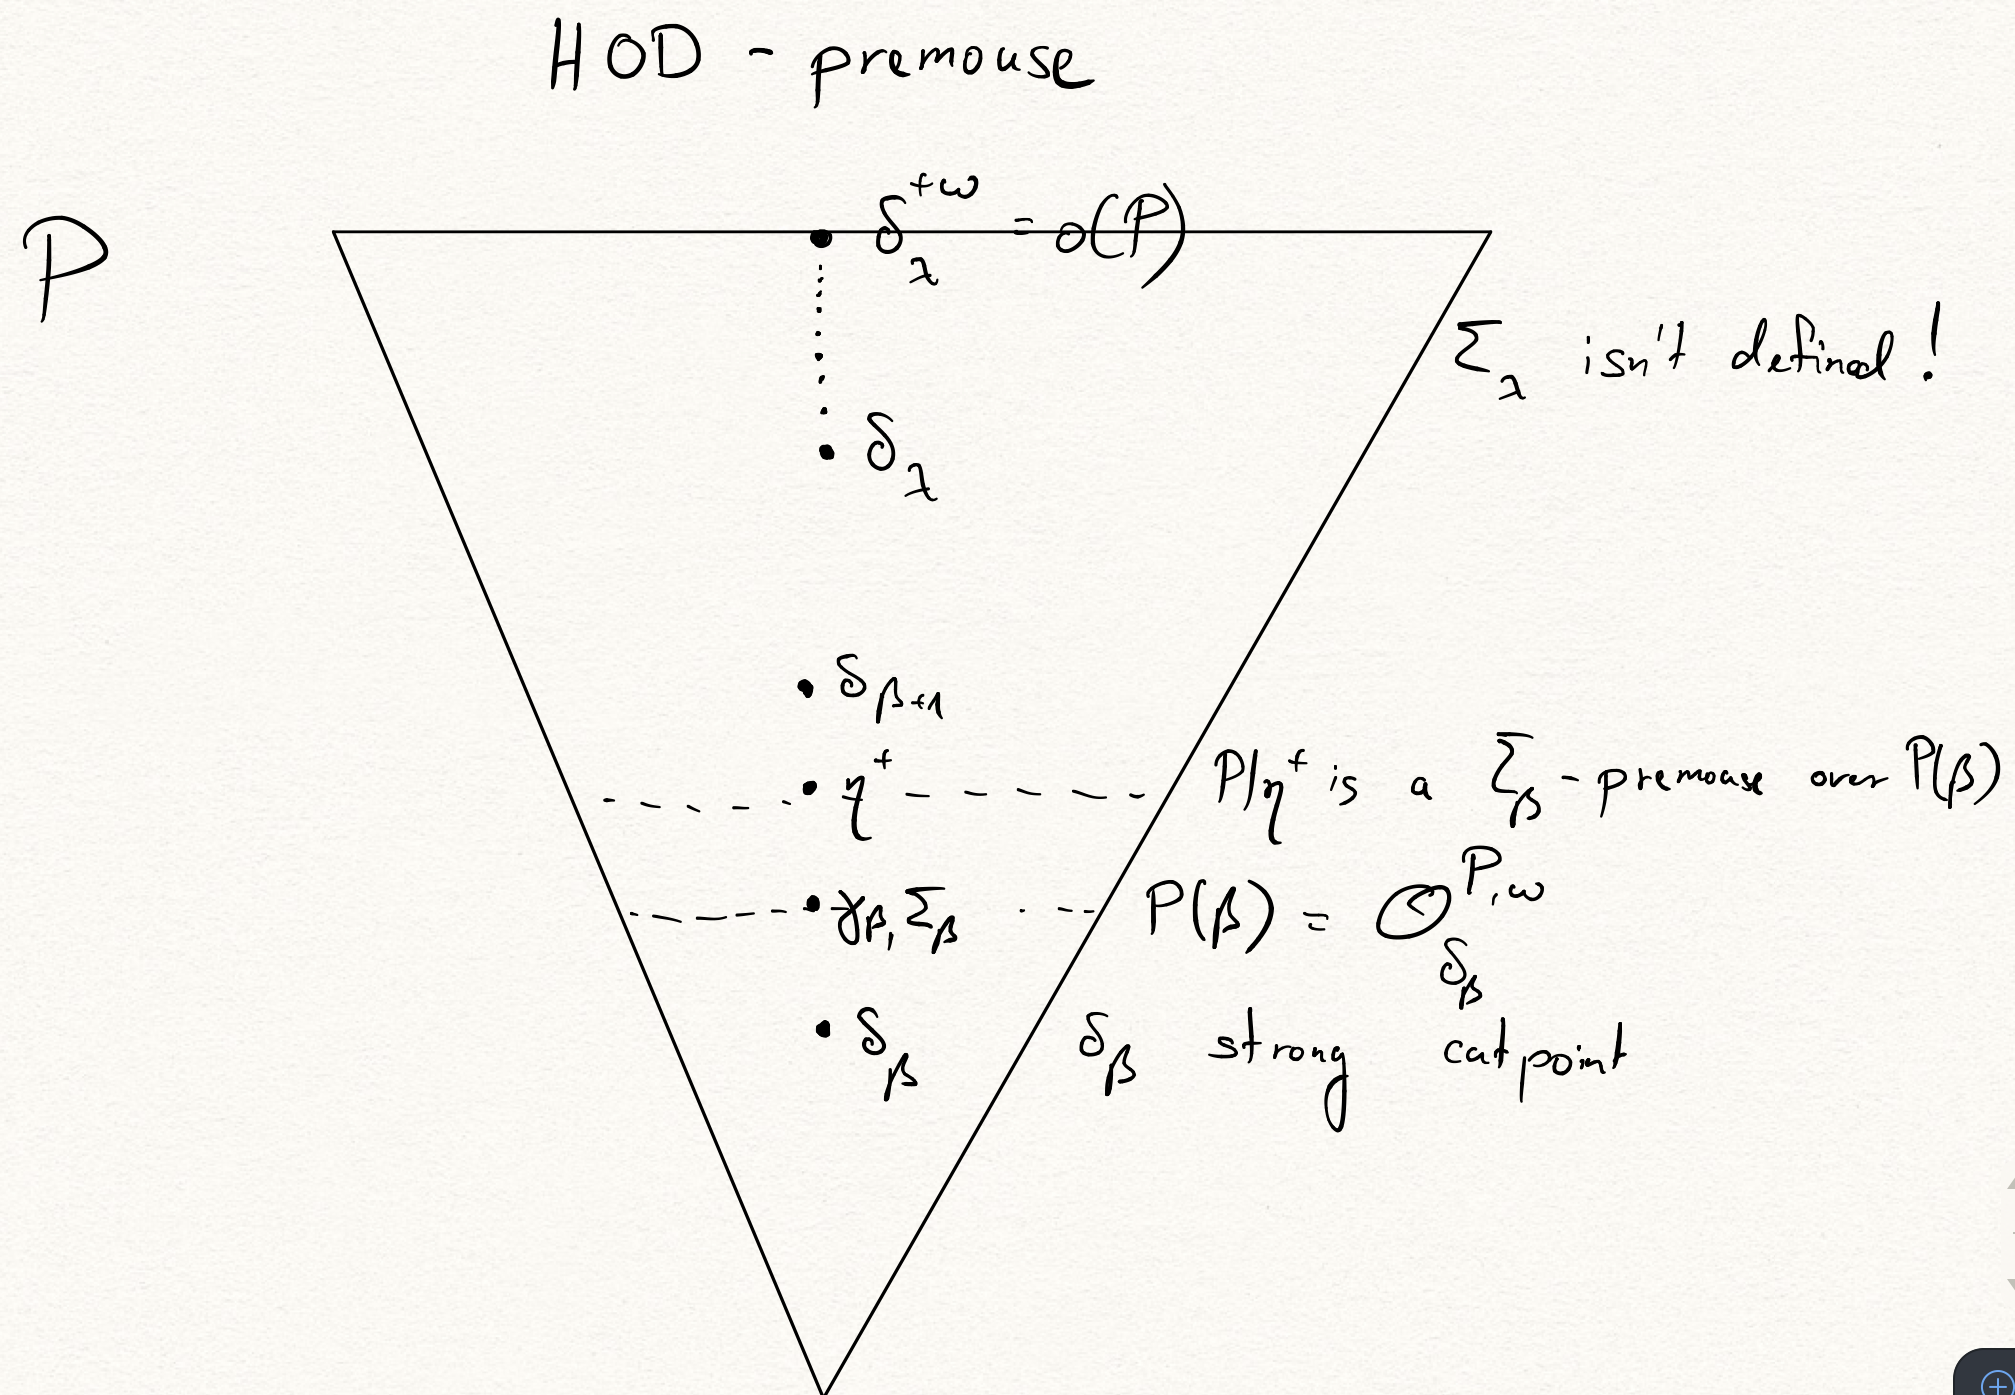
\includegraphics[width=300px]{\string~/gitsky/phd/gfx/hod-premouse.png}
  \caption{$\hod$-premouse}
  \label{fig:hod-premouse}
\end{figure}

\defi{Let $\mathcal{P} = (J^{\vec{E},f}(X); \in, \vec{E}, f, B)$ be a
  $\hod$-premouse. We let \index{$\mathcal{P}^{-}$}
  \[
    \mathcal{P}^{-} =
    \begin{cases}
      P | \gamma_{\lambda^{\mathcal{P}}-1} & \text{, if } \lambda^{\mathcal{P}} \text{ is a successor ordinal,} \\
      \mathcal{P}| \delta^{\mathcal{P}} & \text{, otherwise}.
    \end{cases}
  \]
  See \autoref{fig:P^-}
  \todo[inline]{add picture and figure out why we don`t just let
    $\mathcal{P}^{-} =
    \mathcal{P}(\gamma^{\mathcal{P}}_{\lambda^{\mathcal{P}}-1})$ in
    the successor case.}  }

\begin{figure}
  \centering
  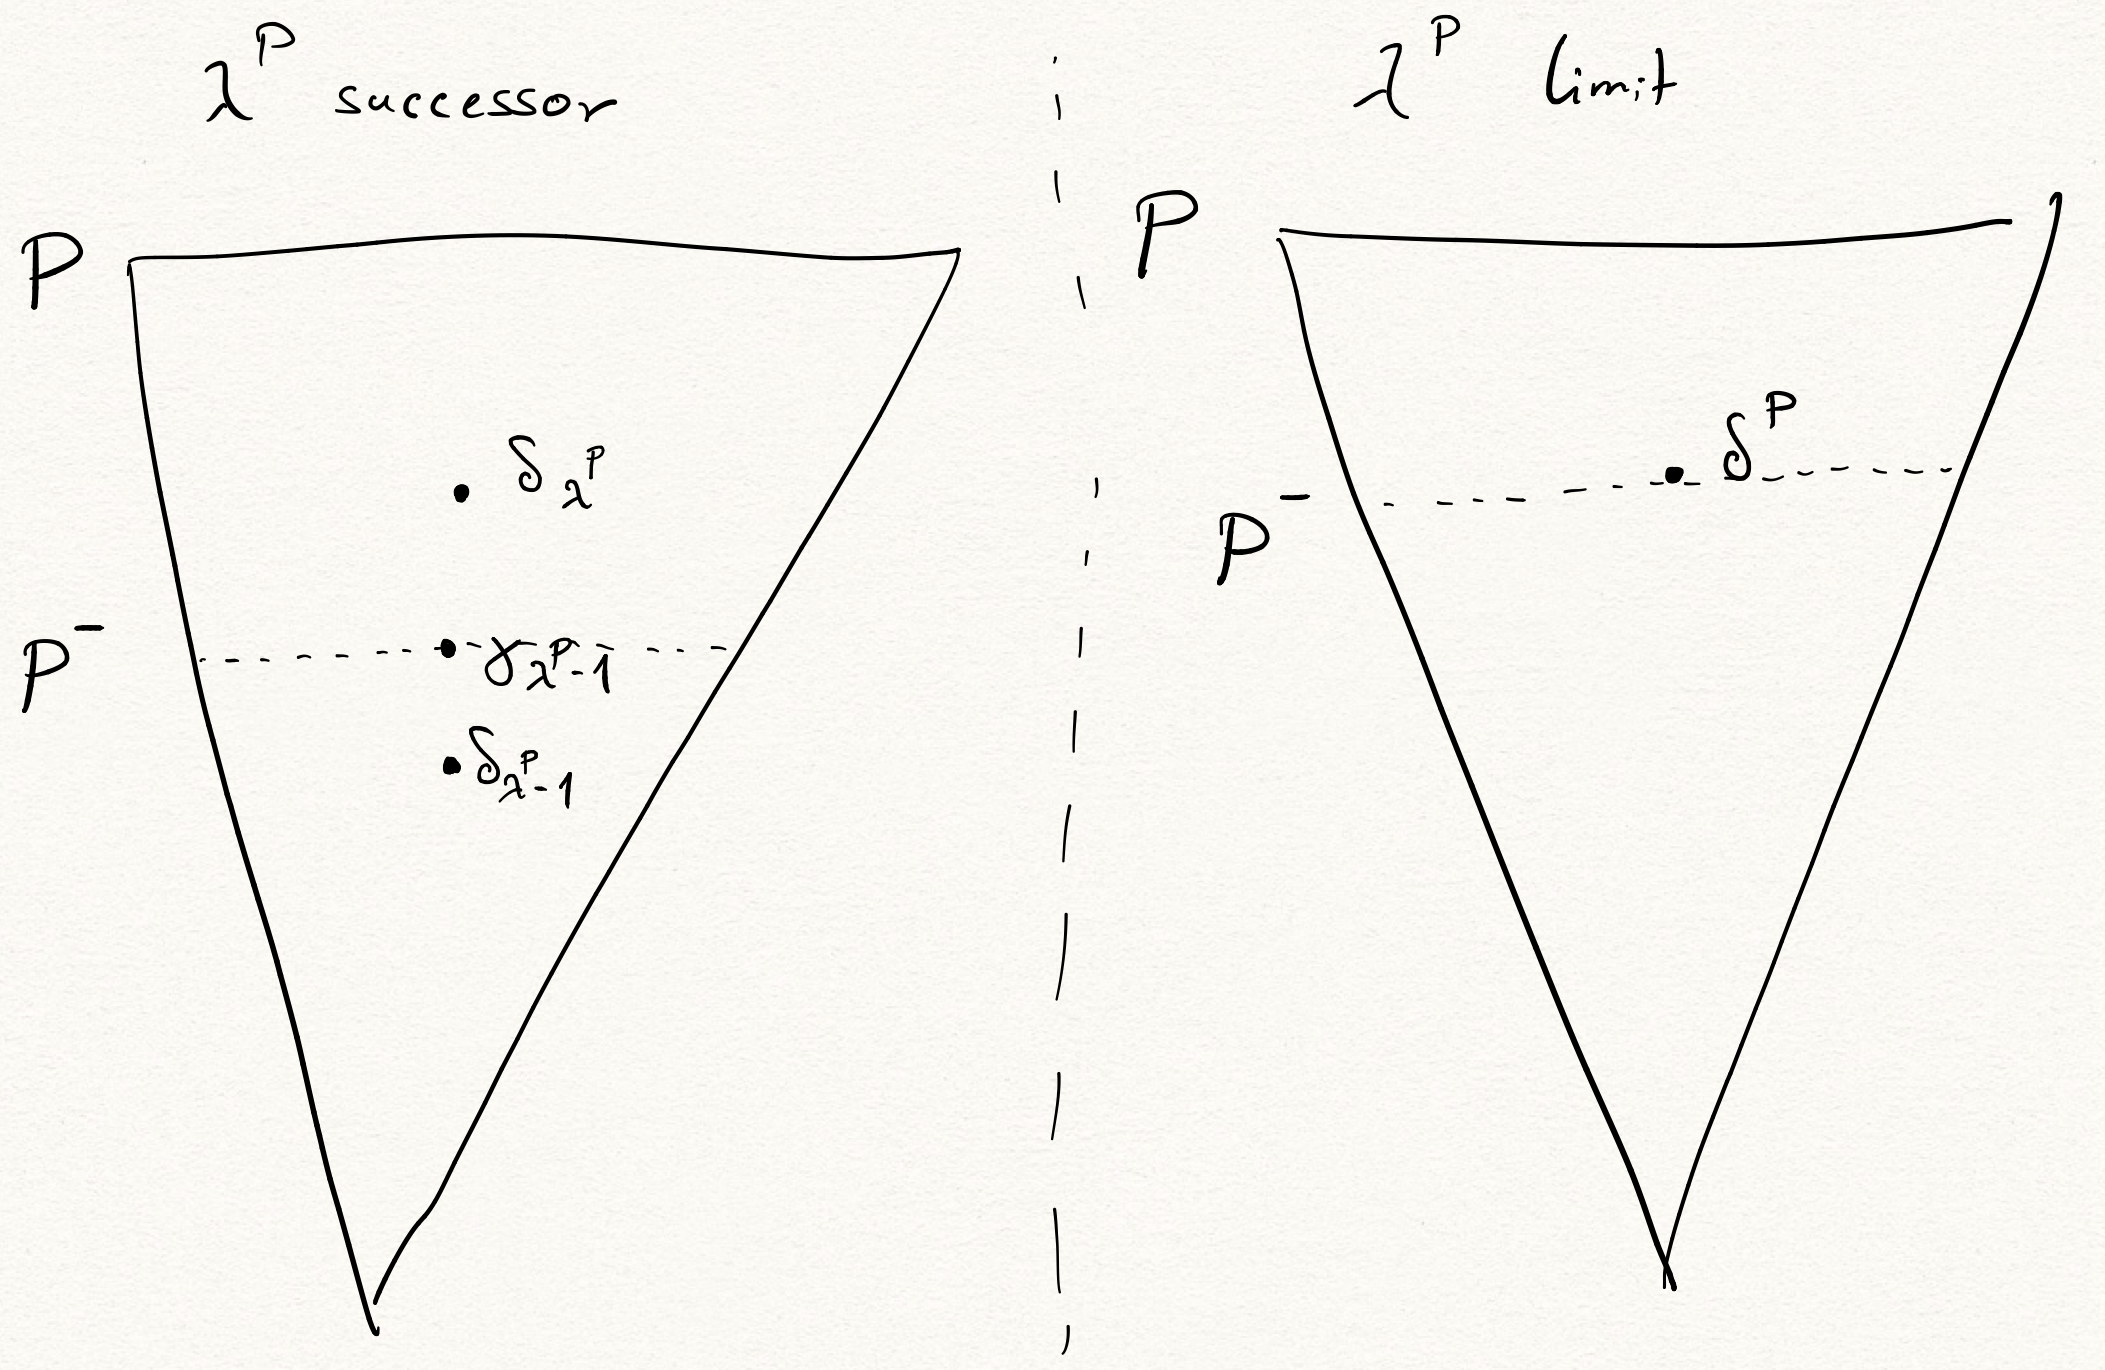
\includegraphics[width=250px]{\string~/gitsky/phd/gfx/P-minus.png}
  \caption{$\mathcal{P}^{-}$}
  \label{fig:P^-}
\end{figure}

\defi{ Let $\mathcal{P}, \mathcal{Q}$ be $\hod$-premice. We write
  $\mathcal{P} \lehod \mathcal{Q}$
  \index{$\mathcal{P} \lehod \mathcal{Q}$} if there is some
  $\alpha \le \lambda^{\mathcal{Q}}$ such that
  $\mathcal{P} = \mathcal{Q}(\alpha)$. We also write
  $\mathcal{P} \lhod \mathcal{Q}$
  \index{$\mathcal{P} \lhod \mathcal{Q}$} if
  $\mathcal{P} \lehod \mathcal{Q}$ and $\mathcal{P} \neq \mathcal{Q}$. \\
  In this case we say that $\mathcal{P}$ is a (proper)
  \textbf{$\hod$-initial segment} \index{$\hod$-initial segment} of
  $\mathcal{Q}$.}

\defi{
  Let $\mathcal{P} = (J^{\vec{E},f}(X); \in, \vec{E}, f, B)$ be a
  $\hod$-premouse and $\alpha \le \lambda^{\mathcal{P}}$.
  \begin{enumerate}
  \item If $\alpha < \lambda^{\mathcal{P}}$, we let
    $\Sigma^{\mathcal{P}}_{\alpha}$
    \index{$\Sigma^{\mathcal{P}}_{\alpha}$} be the internal iteration
    strategy of $\mathcal{P}(\alpha)$ coded by $f(\alpha)$ and
  \item \index{$\Sigma^{\mathcal{P}}_{<\alpha}$}
    $\Sigma^{\mathcal{P}}_{<\alpha} := \bigoplus_{\beta<\alpha}
    \Sigma^{\mathcal{P}}_{\beta}$.
  \end{enumerate}
  We also let $\Sigma^{\mathcal{P}} := \Sigma^{\mathcal{P}}_{< \lambda^{\mathcal{P}}}$.
}

\rema{

  By the agreement of the internal iteration strategies of
  $\hod$-premice (\autoref{defi:agreement of internal iteration
    strategy} in \autoref{defi:hod premouse} \todo{reference broken}),
  $\Sigma^{\mathcal{P}}_{\alpha}$ already includes all of the
  information of $\Sigma^{\mathcal{P}}_{< \alpha}$ and can be
  identified with $\Sigma^{\mathcal{P}}_{< \alpha + 1}$.
  
}

\defi{ Let $\mathcal{P}$ be a $\hod$-premouse. $\Sigma$ is a
  \textbf{$(\kappa,\lambda)$-iteration strategy} \index{iteration
    strategy for $\hod$-premouse} for $\mathcal{P}$ if it is a winning
  strategy for player II in the iteration game
  $\mathcal{G}(\mathcal{P},\kappa,\lambda)$ \todo{add reference} and
  whenever
  $(\vec{\mathcal{T}},\mathcal{Q}) \in I(\mathcal{P}, \Sigma)$, then
  $\mathcal{Q}$ is a $\hod$-premouse such that
  $\Sigma^{\mathcal{Q}} = \Sigma_{\mathcal{Q}, \vec{\mathcal{T}}} \cap
  \mathcal{Q}$.
}

\rema{

  In particular, $\Sigma^{\mathcal{P}} = \Sigma \cap \mathcal{P}$,
  i.e. $\Sigma$ extends the internal iteration strategy of
  $\mathcal{P}$.

}

\defi{
$(\mathcal{P}, \Sigma)$ is a \textbf{$\hod$-pair} \index{$\hod$-pair} if
\begin{enumerate}
\item $\mathcal{P}$ is a $\hod$-premouse and
\item $\Sigma$ is a $(\omega_{1},\omega_{1}+1)$-iteration strategy for
  $\mathcal{P}$ with hull condensation.
\end{enumerate}

\todo[inline]{the definition of hod pair is different in both versions
  of Grigor`s thesis. Verify that this is the intended one.}

}

\subsection{$\hod$ Analysis}

\todo[inline]{gather all the information we need on $\hod$ -- this can
  be found in Grigor`s thesis}

\defi{ Let $(P, \Sigma), (Q, \Lambda)$ be $\hod$-pairs. We let
  $(\mathcal{P}, \Sigma) \ledj (\mathcal{Q}, \Lambda)$ iff
  $(\mathcal{P}, \Sigma)$ loses the coiteration with
  $(\mathcal{Q}, \Lambda)$, i.e. there is a
  $(\mathcal{P}, \Sigma)$-iterate $(\mathcal{T}, R)$ and a
  $(\mathcal{Q}, \Lambda)$-iterate $(\mathcal{U},S)$ such that
  \[
    \mathcal{R} \lehod \mathcal{S} \text{ and } \Sigma_{\mathcal{R},
      \mathcal{T}} = \Lambda_{\mathcal{R}, \mathcal{U}}.
  \]
  We also let $(\mathcal{P}, \Sigma) \ldj (\mathcal{Q}, \Lambda)$ iff
  $(\mathcal{P}, \Sigma) \ledj (\mathcal{Q}, \Lambda)$ and
  $(\mathcal{Q}, \Lambda) \nledj (\mathcal{P}, \Sigma)$.

}

\defi{ Let $(\mathcal{P}, \Sigma)$ be a $\hod$-pair such that $\Sigma$
  has branch condensation and is fullness preserving. We recursively
  define
  $\alpha(\mathcal{P}, \Sigma) := | (\mathcal{P}, \Sigma) |_{\ledj}
  \in \on$  via \eq{ | (\mathcal{P},
    \Sigma) |_{\ledj} = \sup \{ | (\mathcal{Q}, \Lambda) |_{\ledj} + 1
    \mid & (\mathcal{Q}, \Lambda) \text{is a }
    \hod \text{-pair such that } \\
    &\Lambda \text{ has branch
      condensation}  \\
    & \text{and is fullness preserving } \} } }

\rema{
  As in the case of ordinary premice, $\ledj$ (or rather $\ldj$)
  is a wellfounded relation. The interesting question is whether it`s
  total.
}

\theo[Sargsyan]{
  Assume $\ad^{+} + V = L(\mathcal{P}(\mathbb{R}))$. Suppose
  $(\mathcal{P}, \Sigma), (\mathcal{Q}, \Lambda)$ are $\hod$-pairs
  such that both $\Sigma$ and $\Lambda$ have branch condensation and
  are fullness preserving. Then
  $(\mathcal{P}, \Sigma) \ledj (\mathcal{Q}, \Lambda)$ or
  $(\mathcal{Q}, \Lambda) \ledj (\mathcal{P}, \Sigma)$.
  
}

\proof{
  \cite[Theorem~5.10]{sargsyan2015hod}.
}

\theo[Sargsyan]{ Assume $\ad^{+} + V =
  L(\mathcal{P}(\mathbb{R}))$. Suppose
  $(\mathcal{P}, \Sigma), (\mathcal{Q}, \Lambda)$ are $\hod$-pairs
  such that both $\Sigma$ and $\Lambda$ have branch condensation and
  are $\Gamma$-fullness preserving for some pointclass $\Gamma$ which
  is closed under continuous images and preimages. Suppose further
  that there is a good pointclass $\Gamma^{*}$ such that
  $\Gamma \cup \{ \code(\Sigma), \code(\Lambda) \} \subseteq
  \Delta_{\underset{\sim}{\Gamma}^{*}}$ \todo{define
    $\code{\Sigma}$}. Then
  $(\mathcal{P}, \Sigma) \ledj (\mathcal{Q}, \Lambda)$ or
  $(\mathcal{Q}, \Lambda) \ledj (\mathcal{P}, \Sigma)$.  }

\proof{
  \cite[Theorem~2.33]{sargsyan2015hod}.
}

\defi{ Suppose $\Gamma$ is a pointclass closed under Wadge
  reducibility and $(\mathcal{P}, \Sigma)$ is a $\hod$-pair such that
  $\Sigma$ has branch condensation and is $\Gamma$-fullness
  preserving. We let
  \begin{enumerate}
    \item
    $\mathcal{F}(\mathcal{P}, \Sigma) = \{ (\mathcal{Q},
    \Sigma_{\mathcal{Q}}) \mid \mathcal{Q} \in pB(\mathcal{P}, \Sigma)
    \}$ \index{$\mathcal{F}^{+}(\mathcal{P}, \Sigma)$} and
  \item 
    $\mathcal{F}^{+}(\mathcal{P}, \Sigma) = \{ (\mathcal{Q},
    \Sigma_{\mathcal{Q}}) \mid \mathcal{Q} \in pI(\mathcal{P}, \Sigma)
    \}$ \index{$\mathcal{F}(\mathcal{P}, \Sigma)$}.  
  \end{enumerate}
}

\rema{

  By \cite[Corollary~2.44]{sargsyan2015hod} $\Sigma$ is commuting, so
  that $\Sigma_{\mathcal{Q}}$ is indeed well-defined.

}

\defi{ Suppose $\Gamma$ is a pointclass closed under Wadge
  reducibility and $(\mathcal{P}, \Sigma)$ is a $\hod$-pair such that
  $\Sigma$ has branch condensation and is $\Gamma$-fullness
  preserving. Let
  $\mathcal{Q}, \mathcal{R} \in pI(\mathcal{P}, \Sigma) \cup
  pB(\mathcal{P}, \Sigma)$. We let
  $\mathcal{Q} \le^{\mathcal{P},\Sigma} \mathcal{R}$
  \index{$\le^{\mathcal{P},\Sigma}$} if
  \begin{enumerate}
  \item $\mathcal{Q} \in pI(\mathcal{P}, \Sigma)$ and $R \in pI(\mathcal{Q}, \Sigma_{Q})$ or
  \item $\mathcal{Q} \in pB(\mathcal{P},\Sigma)$ and
    $(\mathcal{Q}, \Sigma_{\mathcal{Q}}) \ledj (\mathcal{R},
    \Sigma_{\mathcal{R}})$.
  \end{enumerate}
}

\lemm[Sargsyan]{

  $\le^{\mathcal{P}, \Sigma}$ is directed.

}

\proof{
  \cite[Lemma~4.17]{sargsyan2015hod}.
}


\defi{
  Suppose $\Gamma$ is a pointclass closed under Wadge reducibility and
  $(\mathcal{P}, \Sigma)$ is a $\hod$-pair such that $\Sigma$ has
  branch condensation and is $\Gamma$-fullness preserving. Let
  $\mathcal{Q}, \mathcal{R} \in \piterates(\mathcal{P}, \Sigma) \cup
  \pblowups(\mathcal{P}, \Sigma)$ be such that, for some
  $\alpha \le^{\mathcal{R}}$,
  $\mathcal{R}(\alpha) \in pI(\mathcal{Q}, \Sigma_{\mathcal{Q}})$. We let
  \[
    \pi^{\Sigma}_{\mathcal{Q}, \mathcal{R}} \colon \mathcal{Q} \to \mathcal{R}(\alpha)
  \]
  \index{$\pi^{\Sigma}_{\mathcal{Q}, \mathcal{R}}$}
  be the iteration map given by $\Sigma_{\mathcal{Q}}$. \\
  We let
  \begin{enumerate}
  \item
    $\mathcal{M}_{\infty}(\mathcal{P}, \Sigma) = \dirlim
    (\mathcal{F}(\mathcal{P},\Sigma), \pi^{\Sigma}_{\mathcal{Q},
      \mathcal{R}} \colon \mathcal{Q}, \mathcal{R} \in pB(\mathcal{P},
    \Sigma) \wedge \exists \alpha \le \lambda^{\mathcal{R}}
    \mathcal{R}(\alpha) \in pI(\mathcal{Q}, \Sigma_{\mathcal{Q}}) )$
    \index{$\mathcal{M}_{\infty}(\mathcal{P}, \Sigma)$}
    and
  \item
    $\mathcal{M}^{+}_{\infty}(\mathcal{P}, \Sigma) = \dirlim
    (\mathcal{F}(\mathcal{P},\Sigma), \pi^{\Sigma}_{\mathcal{Q},
      \mathcal{R}} \colon \mathcal{Q}, \mathcal{R} \in pI(\mathcal{P},
    \Sigma) \wedge \mathcal{Q} \le^{\Sigma}_{\mathcal{Q}, \mathcal{R}}
    \mathcal{R})$.
    \index{$\mathcal{M}^{+}_{\infty}(\mathcal{P}, \Sigma)$}
  \end{enumerate}
  For $\mathcal{Q} \in pB(\mathcal{P}, \Sigma)$ and
  $\mathcal{R} \in pI(\mathcal{P}, \Sigma)$ we let
  \begin{enumerate}
  \item
    $\pi^{\Sigma}_{\mathcal{Q}, \infty} \colon \mathcal{Q} \to
    \mathcal{M}_{\infty}(\mathcal{P}, \Sigma)$
    \index{$\pi^{\Sigma}_{\mathcal{Q}, \infty}$} and
  \item
    $\sigma^{\Sigma}_{\mathcal{R}, \infty} \colon \mathcal{R} \to
    \mathcal{M}^{+}_{\infty}(\mathcal{P}, \Sigma)$
    \index{$\sigma^{\Sigma}_{\mathcal{R}, \infty}$}
  \end{enumerate}
  be the direct limit maps.
}

\defi{ Let $(\mathcal{P}, \Sigma)$ be as above. We let
  \begin{enumerate}
  \item $\delta_{\infty}(\mathcal{P}, \Sigma)$
    \index{$\delta_{\infty}(\mathcal{P}, \Sigma)$} be the supremum of
    the Woodin cardinals of
    $\mathcal{M}_{\infty}(\mathcal{P}, \Sigma)$,
  \item $\delta^{+}_{\infty}(\mathcal{P}, \Sigma)$
    \index{$\delta^{+}_{\infty}(\mathcal{P}, \Sigma)$} be the supremum
    of the Woodin cardinals of
    $\mathcal{M}^{+}_{\infty}(\mathcal{P}, \Sigma)$ and
  \item
    $\lambda_{\infty}(\mathcal{P}, \Sigma) :=
    \lambda^{\mathcal{M}^{+}_{\infty}(\mathcal{P}, \Sigma)}$.
    \index{$\lambda_{\infty}(\mathcal{P}, \Sigma)$}
  \end{enumerate}  
}

\lemm[Sargsyan]{
  Let  $\Gamma$ be a pointclass closed under Wadge
  reducibility. Suppose $(\mathcal{P}, \Sigma)$ is a $\hod$-pair such
  that $\lambda^{\mathcal{P}}$ is a limit ordinal and $\Sigma$ has
  branch condensation and is $\Gamma$-fullness preserving. Then
  \begin{enumerate}
  \item $\delta_{\infty}(\mathcal{P}, \Sigma) = \delta^{+}_{\infty}(\mathcal{P}, \Sigma)$ and
  \item $\mathcal{M}^{+}_{\infty}(\mathcal{P}, \Sigma) | \delta^{+}_{\infty} = \mathcal{M}_{\infty}(\mathcal{P}, \Sigma)$.
  \end{enumerate}
}

\proof{
  \cite[Lemma~4.18]{sargsyan2015hod}.
}

\todo[inline]{We will likely not need the entire theorem and
  should reduce it to the part that we need once we are done.}
\theo[Sargsyan]{Assume $\ad^{+}$, let
  $\Gamma \subseteq \mathcal{P}(\mathbb{R})$ be such that
  $\Gamma = \mathcal{P}(\mathbb{R}) \cap L(\Gamma, \mathbb{R})$ and
  $\mathcal{H} = \hod^{L(\Gamma,\mathbb{R})}$. Then the following
  holds:
  \begin{enumerate}
  \item If $L(\Gamma,\mathbb{R}) \models \phi$ \todo{define $\phi$}
    then for all $(\mathcal{P}, \Sigma) \in \Gamma$ such that
    $\alpha(\mathcal{P}, \Sigma) < \Omega^{\Gamma}$ \todo{define
      $\Omega^{\Gamma}$} we have, for all
    $\alpha \le \alpha(\mathcal{P}, \Sigma)$,
    \begin{enumerate}
    \item
      $\delta_{\alpha}^{\mathcal{M}^{+}_{\infty}(\mathcal{P}, \Sigma)}
      = \theta^{\Gamma}_{\alpha}$ \todo{define
        $\theta^{\Gamma}_{\alpha}$} and
    \item
      $\mathcal{M}^{+}_{\infty}(\mathcal{P}, \Sigma) |
      \theta^{\Gamma}_{\alpha} =
      (V^{\mathcal{H}}_{\theta^{\Gamma}_{\alpha}};\in,
      \vec{E}^{\mathcal{M}^{+}_{\infty}(\mathcal{P}, \Sigma)}
      \restriction \theta^{\Gamma}_{\alpha}, \Lambda \restriction
      \theta^{\Gamma}_{\alpha})$,
    \end{enumerate}
    where $\Lambda$ is the iteration strategy coded by
    $f^{\mathcal{M}^{+}_{\infty}(\mathcal{P}, \Sigma)}$.

  \item If $L(\Gamma, \mathbb{R}) \models \psi$ \todo{define $\psi$} then for all $\alpha \le \Omega^{\Gamma}$
    \begin{enumerate}
    \item $\delta_{\alpha}^{\mathcal{M}^{+}_{\infty}(\mathcal{P}, \Sigma)}
      = \theta^{\Gamma}_{\alpha}$ and
    \item
      $\mathcal{M}^{+}_{\infty}(\mathcal{P}, \Sigma) |
      \theta^{\Gamma}_{\alpha} =
      (V^{\mathcal{H}}_{\theta^{\Gamma}_{\alpha}};\in,
      \vec{E}^{\mathcal{M}^{+}_{\infty}(\mathcal{P}, \Sigma)}
      \restriction \theta^{\Gamma}_{\alpha}, \Lambda \restriction
      \theta^{\Gamma}_{\alpha})$.
    \end{enumerate}
  \item Suppose $\Gamma^{*} \subseteq \mathcal{P}(\mathbb{R})$ is such
    that $\Gamma \subseteq \Gamma^{*}$,
    $L(\Gamma^{*}, \mathbb{R}) \models \ad^{+}$ and there is a
    $\hod$-pair $(\mathcal{P}, \Sigma) \in \Gamma^{*}$ such that
    \begin{enumerate}
    \item $\Sigma$ has branch condensation and is $\Gamma$-fullness preserving,
    \item $\lambda^{\mathcal{P}}$ is a successor ordinal,
      $\code(\Sigma_{\mathcal{P}^{-}}) \in \Gamma$ and
      $L(\Gamma, \mathbb{R})$ models that $(\mathcal{P}, \Sigma_{\mathcal{P}^{-}})$ is a suitable pair such that
      $\alpha(\mathcal{P}^{-}, \Sigma_{\mathcal{P}^{-}}) = \alpha$, \todo{define suitable pair}
    \item there is a sequence
      $(B_{i} \mid i < \omega) \subseteq \mathbb{B}(\mathcal{P}^{-},
      \Sigma_{\mathcal{P}^{-}})^{L(\Gamma, \mathbb{R})}$ which guides
      $\Sigma$ and \todo{define $\mathbb{B}(..)$ and what it means to
        be guided}
    \item for any
      $B \in \mathbb{B}(\mathcal{P}^{-},
      \Sigma_{\mathcal{P}^{-}})^{L(\Gamma, \mathbb{R})}$ there is some
      $\mathcal{R} \in \piterates(\mathcal{P}, \Sigma)$ such that
      $\Sigma_{\mathcal{R}}$ respects $B$. \todo{define respects $B$}
    \end{enumerate}
    Then $L(\Gamma, \mathbb{R}) \models \psi$ and
    $\mathcal{M}_{\infty}(\mathcal{P}, \Sigma) =
    \mathcal{M}^{+}_{\infty}(\mathcal{P}, \Sigma)$.
  \end{enumerate}
}

\proof{
  \cite[Theorem~4.24]{sargsyan2015hod}.
}

\section{The tame case}

Define
\eq{
  \Gamma_0:=\{A\subset\mathbb R\mid L(A,\mathbb R)\models\ad+\Omega=0\}.
}

\lemm[$\di$][lemm.lpcontainsgammainfty]{
  $\Gamma_0=\lp(\mathbb R)\cap\p(\mathbb R)$.
}
\proof{
  $(\supset)$ Let $\M\pinit\lp(\mathbb R)$ and let $A\subset\mathbb R$ be an element of $\M$. Since $\M$ projects to $\mathbb R$ and is sound, we get that $A$ is $\od_x$ for a real $x$, so that everything in $L(A,\mathbb R)$ is also ordinal definable in a real as well. Since $\lp(\mathbb R)\models\ad$ we then get that $\ad+\Omega=0$ holds in $L(A,\mathbb R)$, making $A\in\Gamma_0$.\todo{Check this proof.}

  \qquad $(\subset)$ Let $A\in\Gamma_0$. Since we're assuming $\ch$ we get that $V[g]\models|\mathbb R|=\aleph_1^V=\aleph_0$, so fix a generic bijection $b:\omega\to\mathbb R^V$ in $V[g]$. Define $a_b\in\mathbb R$ as $n\in a_b$ iff $b(n)\in A$. As $L(A,\mathbb R)\models\ad+\theta_0=\Theta$ it holds that $A$ is $\od_z^{L(A,\mathbb R)}$ for $z\in\mathbb R$, so that
\eq{
  A=j(A)\cap\mathbb R^V\in\od^{L(j(A),\mathbb R^{V[g]})}_{z,\mathbb R^V}.
}

In particular, as $A$ and $\mathbb R^V$ are definable from $b$ and $a_b$ is definable from $b$, we get that $a_b\in\od^{L(j(A),\mathbb R^{V[g]})}_b$. By $\mc$ we then get that there's some $b$-premouse $\M\in L(j(A),\mathbb R^{V[g]})$ projecting to $b$ with $a_b\in\M$ and a $\Sigma$ such that
\eq{
  L(j(A),\mathbb R^{V[g]})\models\godel{\text{$\Sigma$ is an $\omega_1$-iteration strategy for $\M$}}.
}

\todo[inline]{Why is it that we have to go through $b$ in this fashion? Can't we just use $\mc$ and get $\N$ without going through $\M$? Is it because $L(j(A),\mathbb R^{V[g]})$ doesn't know that $\mathbb R^V$ is countable?}

From this $\M$ we can then get an $\mathbb R^V$-premouse $\N\in L(j(A),\mathbb R^{V[g]})$ projecting to $\mathbb R^V$ with $A\in\N$ and
\eq{
  L(j(A),\mathbb R^{V[g]})\models\godel{\text{$\Sigma$ is an $\omega_1$-iteration strategy for $\N$}}.
}

Now $\N$ is $\od^{L(j(A),\mathbb R^{V[g]})}_{\mathbb R^V}$, and since we don't have divergent models of $\ad^+$ it holds that, letting $\Theta^{j(A)}:=\Theta^{L(j(A),\mathbb R^{V[g]})}$,
\eq{
  V[g]\models L(j(A),\mathbb R)=L(P_{\Theta^{j(A)}}(\mathbb R)).
}

This means that $\N\in\od^{V[g]}_{\mathbb R^V}$, so that homogeneity of $I$ we get that $\N\in V$. It remains to show that $\N\init\lp(\mathbb R^V)$, meaning that we need to show that $\N$ is countably $(\omega_1+1)$-iterable in $V$. But letting $\overline\N\to\N$ be a countable hull in $V$ we get that $j(\overline\N)=\overline\N$, so that elementarity of $j$ implies that $\Sigma\restr V\in V$ \todo{Why's this?} is an $\omega_1^{V[g]}=\omega_2^V$-iteration strategy for $\overline\N$ \todo{Is this really this iterable?} and we're done.
}

\prop[$\di$]{
  $\cof^V(\Theta^{\lp(\mathbb R)})=\omega$.
}
\proof{
  \todo[inline]{See Ketchersid`s Thesis 3.17 or 7.4.2 in the CMI book. Perhaps we don't need it though, following Wilson's thesis.}
}

\theo{
  Let $\Gamma$ be an inductive-like pointclass. If $\M$ is a suitable quasi-iterable premouse, $\A\in[\env(\Gamma)]^\omega$ is closed under recursive join and the $\A$-guided map $\pi_{\M,\infty}^{\A}$ is both total on $\M$ and has the full factors property, then there's a unique $\Gamma$-fullness preserving $(\omega_1,\omega_1)$-strategy $\Phi$ for $\M$ such that, for every quasi-iterate $\P$ of $\M$,
\begin{itemize}
  \item $\P$ is a non-dropping $\Phi$-iterate of $\M$; and
  \item the $\Phi$-iteration map $i:\M\to\P$ equals the $\A$-guided map $\pi_{\M,\P}^{\A}$.
\end{itemize}
}

Let $\Phi_{\M}$ be the unique strategy for $\M$ as in the above theorem. We now improve this to include branch condensation.

\todo[inline]{The 3d argument is quite similar to the proof of Theorem 7.19 in the outline.}

\begin{figure}
  \pix[0.8]{\string~/gitsky/phd/gfx/trangs_pic.png}
  \caption{The three-dimensional argument in Theorem \ref{theo.3d}}
  \label{fig.3d}
\end{figure}

\theo[][theo.3d]{
  Let $\Gamma$ be an inductive-like pointclass and assume that ${\bf\Delta}_\Gamma$ is determined and that $\Gamma$-$\mc$ holds. Let $\M$ be an $\omega$-suitable quasi-iterable premouse such that $\D(\M)\equiv\M_\Gamma$\todo{This is the companion of $\Gamma$, see Trevor's thesis. I'm not sure if we can find $\M$ like this, however.}, let $\A\in[\env(\Gamma)]^\omega$ be closed under recursive join, assume $\pi_{\M,\infty}^{\A}$ is total on $\M$ and that it has the full factors property. Let $\Phi:=\Phi_{\M}$. Then there's a $(\T,\P)\in\iterates(\M,\Phi)$ such that $\Phi_{\U,\Q}$ has $\A$-condensation, and hence also branch condensation, for every $(\U,\Q)\in\iterates(\P,\Phi_{\T,\P})$.
}
\proof{
  Assume not and fix $A\in\env(\Gamma)$ such that given any $(\T,\P)\in\iterates(\M,\Phi)$ there's a $(\U,\Q)\in\iterates(\P,\Phi_{\T,\P})$ such that $\Phi_{\U,\Q}$ doesn't have $A$-condensation. Applying this inductively, we get a sequences $\bra{\Q^0_n,\R^0_n,\T^0_n,\pi^0_n,\sigma^0_n,j^0_n\mid n<\omega}$ such that
\begin{enumerate}
  \item $\Q^0_0:=\M$;
  \item $\pi^0_n:\Q^0_n\to\Q^0_{n+1}$ is the iteration map through a tree of successor length, according to $\Phi$;
  \item $\sigma^0_n:\Q^0_n\to\R^0_n$ an iteration map through a tree of limit length, according to $\Phi$;
  \item $j^0_n:\R^0_n\to\Q^0_{n+1}$ is elementary such that $\pi^0_n=j^0_n\circ\sigma^0_n$;
  \item $(j^0_n)^{-1}(\tau^{\Q^0_{n+1}}_{A,j^0_n(\kappa)})\neq\tau^{\R^0_n}_{A,\kappa}$ for every $\R^0_n$-cardinal $\kappa\geq\delta_0^{\R^0_n}$.\\
\end{enumerate}

  Let $\Q^0_\omega$ be the direct limit of the $\Q^0_n$'s under the $\pi^0_n$ maps. Also let $\bra{x_n\mid n<\omega}$ enumerate the reals of $\M_\Gamma$ and pick $s\in[\on]^{<\omega}$ and a formula $\varphi$ such that
\eq{
  \forall x\in\mathbb R(x\in A\Leftrightarrow\M_\Gamma\models\varphi[x,s]).
}

Our strategy now is now firstly to capture all the $x_n$'s so that the derived models of the resulting structures become equal to $\M_\Gamma$. See Figure \ref{fig.3d}.

  \qquad Perform a genericity iteration of $\Q^0_0$ above $\delta_0^{\Q^0_0}$ to $\Q^1_0$ to make $x_0$ generic over $\Q^1_0$ at $\delta_1^{\Q^1_0}$, while lifting the genericity iteration tree via the copy construction to the $\Q^0_n$'s and $\R^0_n$'s, and picking branches on the genericity iteration tree on $\Q^0_0$ by using $\Phi_{\Q^0_\omega}$ on the lifted tree on $\Q^0_\omega$. Let $\tau^0_0:\Q^0_0\to\Q^1_0$ be the genericity iteration map and $\W_0$ the last model of the lifted tree on $\Q^0_\omega$.

  \qquad Now perform another genericity iteration of the last model of the lifted iteration tree on $\R^0_0$ above its $\delta_0$ to $\R^1_0$ to make $x_0$ generic over $\R^1_0$ at $\delta_1^{\R^1_0}$, with branches being picked by lifting the iteration tree to $\W_0$ and using the branches according to $\Phi_{\W_0}$. Let $k^0_0:\R^0_0\to\R^1_0$ be the iteration embedding, $\sigma^1_0:\Q^1_0\to\R^1_0$ be the shift of $\sigma^0_0$ followed by latter genericity iteration, and $\W_1$ the last model of the lifted tree on $\W_0$.

  \qquad Do a third genericity iteration of the last model of the lifted stack on $\Q^0_1$ above its $\delta_0$ to $\Q^1_1$ to make $x_0$ generic at $\delta_1^{\Q^1_1}$, with branches being picked by lifting the tree to $\W_1$ and using branches picked by $\Phi_{\W_1}$. Let $\tau^0_1:\Q^0_1\to\Q^1_1$ be the iteration embedding, $j^1_0:\Q^1_0\to\R^1_1$ be the natural map, and $\pi^1_0:=j^1_0\circ\sigma^1_0$.

  \qquad Now continue this process to make $x_0$ generic over the $\Q^0_n$'s and $\R^0_n$'s, and let $\Q^1_\omega$ be the direct limit of the $\Q^1_n$'s under the $\pi^1_n$ maps. Then start at $\Q^1_0$ and repeat the same thing to make $x_1$ generic at the respective $\delta_2$'s and so on. Let $\Q^\omega_i$ be the direct limit of the $\Q^n_i$'s under the $\tau^n_i$ maps, $\R^\omega_i$ the direct limit of the $\R^n_i$'s under the $k^n_i$ maps and $\Q^n_\omega$ the direct limit of the $\Q^n_i$'s under the $\pi^n_i$ maps.

  \qquad By construction we get that the $\pi^0_n$'s and $\tau^n_\omega$'s are all by $\Phi$ and its tails, and that $\Q^\omega_\omega$ is wellfounded and $\lp^\Gamma$-full, so that the $\Q^\omega_n$'s and the $\R^\omega_n$'s are also wellfounded and $\lp^\Gamma$-full.

\clai{
  \label{clai.fix_s}
  There exists some $k<\omega$ such that $\pi^\omega_n$ fixes $s$ for every $n\geq k$.
}

\begin{figure}
  \pix[0.5]{\string~/gitsky/phd/gfx/fix_s.png}
  \caption{The argument in Claim \ref{clai.fix_s}.}
  \label{fig.fix_s}
\end{figure}

\cproof{ It suffices to show that
  $(\pi^{\omega}_{n}(\xi) \mid n < \omega)$ is eventually constant for
  all $\xi \in s$. Suppose this isn`t the case. Fix $\xi \in s$ and a
  strictly increasing sequence $(i_{n} \mid n < \omega)$ such that
  $\pi^{\omega}_{i_{n}}(\xi) > \xi$ for all $n < \omega$. For
  $m < n < \omega$ we then have

  \eq{
    \pi^{\omega}_{i_{m}, \infty}(\xi) = \pi^{\omega}_{i_{n}, \infty}
    \circ \pi^{\omega}_{i_{m}, i_{n}}(\xi) \ge \pi^{\omega}_{i_{n}, \infty}
    \circ \pi^{\omega}_{i_{m}}(\xi) > \pi^{\omega}_{i_{n},
      \infty}(\xi),
  }
  
  so that
  $(\pi^{\omega}_{i_{n}}(\xi) \mid n < \omega)$ is a strictly
  decreasing sequence of ordinals in $\mathcal{Q}^{\omega}_{\omega}$
  -- contradicting its wellfoundedness.  See \autoref{fig.fix_s}.
}

Let $k<\omega$ be as in the claim, and note that the $j^\omega_n$'s also fix $s$ for $n\geq k$. Since $\D(\R^\omega_n)=\M_\Gamma$ for every $n<\omega$, the $\Q^\omega_n$'s and the $\R^\omega_n$'s have uniform definitions for the term relations for $A$ when $n\geq k$, yielding that $j^\omega_n$ pulls back the term relation correctly whenever $n\geq k$, $\contr$.
}

\theo[$\di^+$]{
  $\lp(\mathbb R)\models\godel{\text{there's a fullness preserving hod pair below $\omega_1$}}$.
}
\proof{
  \todo[inline]{Show the above requirements in Wilson's theorem is satisfied? Double check the statement.}
}

\theo[$\di^+$]{
  There is a model $M$ containing all the reals such that $M\models\ad^{+}+\theta_0<\Theta$.
}
\proof{
  \todo[inline]{Let $(\M,\Sigma)$ be a fullness preserving hod pair in $\lp(\mathbb R)$ given by the above theorem. Then $\Sigma\notin\lp(\mathbb R)$ by the proof of 7.4.3 in the CMI book, and in particular $\Sigma\notin\Gamma_0$. Then $M:=L(\Sigma,\mathbb R)$ is the wanted model.}
}



\section{The successor case}

\defi{
  \index{Hod mouse!Extension of a hod mouse}
  Let $(\P,\Sigma)$ and $(\Q,\Lambda)$ be hod pairs below $\omega_1$. We then say that $(\Q,\Lambda)$ \textbf{extends} $(\P,\Sigma)$, or is an \textbf{extension} of $(\P,\Sigma)$, if there exists some $\alpha<\lambda^{\Q}$ such that
  \begin{enumerate}
    \item $\Q(\alpha)\in pI(\P,\Sigma)$; and
    \item $\Sigma_{\Q(\alpha)}=\Lambda_{\Q(\alpha)}$.
  \end{enumerate}

We say that $(\P,\Sigma)$ \textbf{can be extended} if there exists an extension of $(\P,\Sigma)$.
}

\theo[$\di^+$]{
  Every hod pair below $\omega_1$ can be extended.
}

Rough steps in the proof:
\begin{enumerate}
  \item Show that $M_1^{\sharp,\Sigma}$ exists
  \item $\lp^\Sigma(\mathbb R)\models\ad^+$ for some appropriate
    definition of $\lp^\Sigma(\mathbb R)$
  \item The $\Omega>0$ argument should show that there's an
    $A\notin\lp^\Sigma(\mathbb R)$ such that
    $L(A,\mathbb R)\models\ad^+$ and $\Sigma <_W A$
  \item Show $L(A,\mathbb R)$ then has the desired $(\Q,\Lambda)$
    (this step has already been done and can be black boxed)
\end{enumerate}

\section{The limit case}

\theo[$\di^+$]{
  Assume there exists a sequence of hod pairs $(\P_\alpha,\Sigma_\alpha)$ below $\omega_1$ with $(\P_{\alpha+1},\Sigma_{\alpha+1})$ extending $(\P_\alpha,\Sigma_\alpha)$ for every $\alpha$. Then either
  \begin{enumerate}
    \item There exists a hod pair $(\h,\Lambda)$ below $\omega_1$ such that $\lambda^{\h}=\sup_\alpha\lambda^{\P_\alpha}$; or
    \item There exists an $\M$ containing all the reals such that $\M\models\ad_{\mathbb R}+\Theta\text{ is regular}$.
  \end{enumerate}
}

Rough steps in the proof:
\begin{enumerate}
  \item Do the easier countable cofinality case

  \item Coiterate all the hod pairs to some $(\P,\Sigma)$, which has $\lambda:=\lambda^{\P}=\sup_\alpha\lambda^{\P_\alpha}$

  \item If $\lambda$ has non-measurable cofinality then $(\P,\Sigma)$ is the hod pair that we're looking for, so assume this is not the case

  \item Take the derived model $\D(\P,\lambda)$, which then satisfies $\ad_{\mathbb R}+\dc+\Omega=\lambda$, where $\dc$ is because $\lambda$ has uncountable cofinality

  \todo[inline]{This is wrong, as we can't take this derived model. Instead we should form a directed system of all ``nice'' hod pairs having $\lambda$'s below $\lambda^{\P}$ and take the $\lp$-closure of that, which should then be an initial segment of hod; call it $\h$.}

  \item Show that
    $\h|\delta^{\h}$ is the union of $M_\infty^\alpha$ for
    $\alpha<\lambda$, where $M_\infty^\alpha$ is the hod limit of
    \eq{
      \F_\alpha:=\{(\Q,\Psi)\mid\ult(V,g)\models\godel{\text{$(\Q,\Psi)$ is a hod pair and $\lambda^{\Q}=\alpha$}}\}.\footnote{This makes sense because every $M_\infty^\alpha$ is an initial segment of $\h$.}
    }

    Let $\Phi$ be the join of the strategies of the
    $M_\infty^\alpha$'s and show that
    $\h=\lp^\Phi_\omega(\h|\delta^{\h})$.

  \item Show that $\h\models\godel{\text{$\delta^{\h}$ is
        singular}}$, since otherwise
    $\D(\h,\delta^{\h})\models\ad_{\mathbb R}+\Theta\text{ is
      regular}$ and we're done.

  \item We want to construct a strategy $\Lambda$ for $\h$ such that
    $(\h,\Lambda)$ is a hod pair below $\omega_1$, as then this is
    the hod pair that we're looking for.

\end{enumerate}

\defi{ Let $(\mathcal{P}, \Sigma)$ be a hod pair. We let
  \begin{enumerate}
  \item
    $\iterates(\mathcal{P}, \Sigma) := \{ (\vec{\mathcal{T}},
    \mathcal{Q}) \mid \vec{\mathcal{T}} \text{ is a stack on }
    \mathcal{P} \text{ via } \Sigma \text{ with last model }
    \mathcal{Q} \text{ such that } \pi^{\vec{\mathcal{T}}} \text{
      exists} \}$ be the collection of
    \textbf{$(\mathcal{P}, \Sigma)$-iterates} \index{Iterates
      $\iterates(\mathcal{P},
      \Sigma)$}\index{$\iterates(\P,\Sigma)$}\index{Hod mouse!Iterates of
      a hod pair $\iterates(\P,\Sigma)$},
  \item
    $\piterates(\mathcal{P}, \Sigma) := \{ \mathcal{Q} \mid
    (\vec{\mathcal{T}}, \mathcal{Q}) \in \iterates(\mathcal{P},
    \Sigma) \text{ for some } \vec{\mathcal{T}} \}$
    \index{$\piterates(\mathcal{P}, \Sigma)$},
  \item
    $\blowups(\mathcal{P}, \Sigma) := \{ (\mathcal{T},
    \mathcal{M}) \mid \mathcal{M} \lhod \mathcal{Q} \text{ and }
    (\vec{\mathcal{T}}, \mathcal{Q}) \in \iterates(\mathcal{P},
    \Sigma) \}$ be the collection of
    \textbf{$(\mathcal{P}, \Sigma)$-blowups} \index{Blowups
      $\blowups(\P,\Sigma)$} \index{$\blowups(\P,\Sigma)$}\index{Hod
      mouse!Blowups of a hod pair $\blowups(\P,\Sigma)$} and
  \item $\pblowups(\mathcal{P}, \Sigma) := \{ \mathcal{Q} \mid
    (\vec{\mathcal{T}}, \mathcal{Q}) \in \blowups(\mathcal{P},
    \Sigma) \text{ for some } \vec{\mathcal{T}} \}$. \index{$\pblowups(\mathcal{P}, \Sigma)$}
  \end{enumerate}
}

\defi{ Let $(\mathcal{P}, \Sigma)$ be a hod pair and $\Gamma$ is a
  pointclass closed under Boolean operations and continuous images
  and preimages. Then $\Sigma$ is \textbf{$\Gamma$-fullness
    preserving} \index{$\Gamma$-fullness preserving} if for all
  $(\vec{\mathcal{T}}, \mathcal{Q}) \in I(\mathcal{P}, \Sigma)$,
  $\alpha + 1 \le \lambda^{\mathcal{Q}}$ and
  $\delta_{\alpha}^{\mathcal{Q}} < \eta$ which is a strong cutpoint of
  $\mathcal{Q}(\alpha+1)$ we have
  \begin{enumerate}
  \item
    $\mathcal{Q} | \eta^{+ \mathcal{Q}(\alpha + 1)} = \lp^{\Gamma,
      \Sigma_{\mathcal{Q}(\alpha), \vec{\mathcal{T}}}}(\mathcal{Q}
    | \eta)$ and
  \item
    $\mathcal{Q} | \delta_{\alpha}^{+ \mathcal{Q}} = \lp^{\Gamma,
      \oplus_{\beta < \alpha} \Sigma_{\mathcal{Q}(\beta+1)},
      \vec{\mathcal{T}}}(\mathcal{Q}(\alpha))$.
  \end{enumerate}
  $\Sigma$ is \textbf{fullness preserving} \index{fullness preserving}
  iff it is $\mathcal{P}(\mathbb{R})$-fullness preserving.
  \todo{Provide a motivation for this definition.}
  
}



\lemm{
  \todo{This will be useful in the proof of the $A$-condensing lemma.}
  Let $M,N$ be transitive models of $\zfc^{-}$ with largest cardinals
  $\delta^{M}, \delta^{N}$ respectively. Let $\pi \colon M \to N$ be
  an elementary embedding, $\kappa := \crit(\pi)$ and let $E$ be the
  long $(\kappa, \delta^{N})$-extender derived from $\pi$. Then
  $N = \ult(M; E)$ and $\pi = \pi_{E}$ is the canonical ultrapower
  embedding.  }


\proofretard{
  We have the following commutative diagram
  
  \begin{center}
    % Feel free to replace this with a cd diagram instead
    \begin{tikzcd}[row sep=large, column sep=large]
      M \arrow[rrdd, "\pi_{E}"] \arrow[rr, "\pi"] & & N \\
      & & \\
      & & \ult(M;E) \arrow[uu, "k"]
    \end{tikzcd}
  \end{center}

  where $k$ satisfies $k \restriction \delta^{N} = \id$.  Let
  $\delta^{\ult(M; E)}$ be the largest cardinal of $\ult(M;E)$. By
  elementarity $k(\delta^{\ult(M;E)}) = \delta^{N}$, so that
  $\delta^{\ult(M;E)} \le \delta^{N}$. If
  $\delta^{\ult(M;E)} < \delta^{N}$, then
  $k \restriction \delta^{N} = \id$ yields
  $k(\delta^{\ult(M;E)}) = \delta^{\ult(M;E)} < \delta^{N}$, which is
  absurd. Hence $\delta^{\ult(M;E)} = \delta^{N}$ and
  $k \restriction (\delta^{\ult(M;E)} + 1) = \id$. Since
  $\delta^{\ult(M;E)}$ is the largest cardinal of $\ult(M;E)$, it
  follows that $k$ doesn`t have a critical point. Therefore $k = \id$,
  $N = \ult(M;E)$ and $\pi = \pi_{E}$.  $\qed$}

\begin{figure}
  \centering
  \begin{tikzcd}[row sep=large, column sep=large]
      & & j(\h) \\
      & & \\
      \h \arrow[rr, "\pi"] \arrow[uurr, "j"] & & \R \arrow[uu, "\tau"]
    \end{tikzcd}
  \caption{Full Factors Property}
  \label{fig:full factors property}
\end{figure}

\lemm{
  \label{lemm.ff}
  \index{Full factors property}
  $j\restr\h$ has the \textbf{full factors property}\footnote{This terminology was introduced in \cite{Wilson}; in \cite{GrigorUB} this was called \textit{weak condensation}.}, meaning that whenever $\R$ \todo[inline]{$R$ has to be countable in $V[g]$. How can we ensure that, as this only gives that it has size $\leq\aleph_1$? Do we have to resort to the (long) claim in Grigor's uB paper?} is a hod premouse and there are elementary embeddings $\pi:\h\to\R$ and $\tau:\R\to j(\h)$ such that $j\restr\h=\tau\circ\pi$, then $\R$ is $\Sigma^2_1(j(\Omega)^\tau)$-full.
}

\proofretard{
  Let $\Psi:=j(\Omega)^\tau$ and assume the lemma fails, meaning that we have a hod mouse $\R$ and elementary embeddings $\pi:\h\to\R$ and $\tau:\R\to j(\h)$ such that $j\restr\h=\tau\circ\pi$ and $\R\neq\lp_\omega^{\Psi}(\R|\delta^{\R})$, witnessed without loss of generality by an $\M\init\lp^{\Psi}(\R|\delta^{\R})$ such that $\rho(\M)=\delta^{\R}$ and which is not an initial segment of $\R$.
\cd{
  (\h,\Omega) \ar[rr]^\pi \ar[drr]_{j\restr\h} && (\R,\Psi) \ar[d]^\tau \\
  && (j(\h),j(\Omega))
}

  We can then fix some hod pair $(\S^*,\Lambda^*)$ such that $\tau``\R|\delta^{\R}\subset\ran(\pi_{\S^*, \infty}^{\Lambda^*})$, and furthermore let $\xi\leq\lambda^{\S^*}$ be least such that $\tau``\R|\delta^{\R}\subset\ran(\pi_{\S^*(\xi), \infty}^{\Lambda^*})$. Lastly let $(\S,\Lambda)$ be an extension of $(\S^*,\Lambda^*)$ such that $\lambda^{\S}$ is a limit ordinal.

  \todo[inline]{Argue why $\S^*$ and $\S$ exist; we should be in the limit case to argue that $\S$ exists.}

  \qquad Let $\sigma:\R|\delta^{\R}\to\S|\delta_\gamma^{\S}$, where $\S^*(\xi)$ iterates to $\S(\gamma)$, be given by $\sigma(x)=y$ iff $\tau(x)=\pi^{\Lambda}_{\S(\gamma),\infty}(y)$.
\cd{
  (\R|\delta^{\R}, \Psi) \ar[rr]^\tau \ar[dr]_\sigma && (j(\h)|\delta^{j(\h)}, j(\Omega))\\
  & (S|\delta_\gamma^{\S}, \bigoplus_{\beta<\gamma}\Lambda_{\S(\beta)}) \ar[ur]_{\pi^\Lambda_{\S(\gamma),\infty}}
}

We can fix some hod pair $(\S',\Lambda')$ such that\todo{This should follow from generation of good pointclasses.}
\eq{
  L(\Lambda',\mathbb R)\models\godel{\text{$\M$ is a $\Psi$-mouse}}.
}

  By coiterating \todo{This requires us to work in an $\ad^+$ model, so we better assume that somewhere.} $\S$ and $\S'$ we may assume without loss of generality that $\S=\S'$.

\clai{
  There exists a hod pair $(\Q,\Phi)$ such that $\lambda^{\Q}$ is a limit ordinal and $L(\Gamma(\Q,\Phi),\mathbb R)\models\godel{\text{$\M$ is a $\Psi$-mouse}}$.
}

\cproof{
  \todo[inline]{This claim shouldn't be needed, as we should be able to take $\Q$ to be $\S$ in our case, using facts about the $\Gamma$-pointclasses. Also ensure that $\Q\supset\h$, which is possible as we're stretching by $j$.}
}

Fix $(\Q,\Phi)$ as in the claim and let $\N$ be some mouse such that $\M\pinit\N$ and $\N$ has $\omega$ many Woodins on top of $\M$.

\todo[inline]{Explain how this is done. In Grigor's paper he's using that ``$j(\eta)$ is closed under hybrid $\N_\omega$-operators''. In our measurable cofinality case there might be enough room to get this. Postpone until later, when we have an idea of how much operator closure we have at this point.}

Then we get that

\todo[inline]{Why is $\Gamma(\Q,\Phi)$ in $\D(\N)$?}

\eq{
  \D(\N)\models\godel{L(\Gamma(\Q,\Phi),\mathbb R)\models\godel{\text{$\M$ is a $\Psi$-mouse which isn't an initial segment of $\R$}}}.
}

Now throw everything in sight into a countable hull\todo{In $V[g]$, I guess.}, so that
\eq{
  \D(\overline{\N})\models\godel{L(\Gamma(\overline{\Q},\overline{\Phi}),\mathbb R)\models\godel{\text{$\M$ is a $\overline{\Psi}$-mouse which isn't an initial segment of $\R$}}}.
}

\todo[inline]{I think that now $\overline\Q$ are taking the role of ``$L[\T,\h]$'', as Grigor's paper seems to indicate that $\h\subset\overline\Q$.}

Now lift $\pi$ to the ultrapower map $\pi^+$ given by the $(\delta^{\h},\delta^{\R})$-extender over $\overline\Q$ derived from $\pi$, and let $\R^+$ be the ultrapower. Lift also $\sigma,\tau$ to corresponding $\sigma^+,\tau^+$.\todo{A it hand-wavy.}
\cd{
  (\overline{\Q}, \overline{\Phi}) \ar[rr]^{\pi^+} \ar[drr]_{\sigma^+} && (\R^+, \Phi^{**}) \ar[d]^{\tau^+}\\
  && (j(\overline\Q), \Phi^*)
}

\qquad Let now $\Phi^*:=j(\overline{\Phi})$ and $\Phi^{**}:=(\Phi^*)^{\tau^+}$, which is then a strategy for $\R^+$. Since $\overline\Phi=(\Phi^{**})^{\pi^+}$\todo{Check this --- might be by definition of pullback consistency, which is implied by hull condensation.} we get that

\todo[inline]{In Grigor's uB paper he uses a certain derived model $C$ instead of $\D(\overline\N)$, but I can't see how they're different from each other. Also, figure out why the following inclusion is true (it's probably folklore).}

\eq{
  \D(\overline\N)\subset\D(\R^+,\Phi^{**}),
}

implying that\todo{Note sure what's going on here.}
\eq{
  L(\Gamma(\R^+,\Phi^{**}),\mathbb R)\models\godel{\text{$\M$ is a $\Psi$-mouse which isn't an initial segment of $\R$}}.
}

Because $\R^+$ is a $\Psi$-mouse over $\R|\delta^{\R}$, it follows that\todo{Why's that?}
\eq{
  \D(\R^+)\models\godel{\text{$\M$ is a $\Psi$-mouse which isn't an initial segment of $\R$}},
}

which then implies that $\M\in\R^+$, so that $\M\init\R$, a contradiction.\todo{I don't see how this last argument works.}
}$\qed$

\defi{ For every $X\in\P_{\omega_1}(j(\h))$ define
  $Q_X:=\chull^{j(\h)}(X)$ and let
  \[
    \tau_X \colon Q_X\to j(\h)
  \]
  be the uncollapse. \\

  Say that $Y\in\P_{\omega_1}(j(\h)|\delta^{j(\h)})$ \textbf{extends}
  $X$ if $X\cap j(\delta^{\h})\subset Y$ and in that case let
  \begin{enumerate}
  \item $\tau_{X, Y}:=\tau_{X \cup Y}$,
  \item $\Phi_{X,Y}:=j(\Phi)^{\tau_{X,Y}}$,
  \item $Q_{X,Y}:=Q_{X\cup Y}$ and
  \item $\pi_{X,Y} \colon Q_X\to Q_{X,Y}$ is the induced embedding
    given by
    \eq{
      \pi_{X,Y}(x) = \tau_{Y}^{-1}(\tau_{X}(x)).
    }
    % I don`t think we need $\pi_{X,Y,Z}$ but I will leave it here for
    % now, so we can add it back easily
  % \item $\pi_{X,Y,Z}:Q_{X,Y}\to Q_{X,Z}$ is the induced embedding for
  %   $Z \in \P_{\omega_1}(j(\h)|\delta^{j(\h)})$ extending $X \cup Y$.
  \end{enumerate}

  Furthermore define $T_{X}(A)$ for $A \in Q_X\cap\P(\delta^{Q_X})$ as
  \eq{
    T_{X}(A)
    :&= \{ (\varphi,s) \mid \text{$\varphi$ is a formula,
      $s\in[\delta^{Q_{X}}]^{<\omega}$ and
      $Q_X\models\varphi[s,A]$} \} \\
    &= \{ (\varphi,s) \mid \text{$\varphi$ is a formula,
      $s\in[\delta^{Q_{X}}]^{<\omega}$ and
      $j(\h)\models\varphi[\tau_X(s),\tau_X(A)]$}\} }

  and let $T_{X,Y}(A)$ be given as
  \eq{
    T_{X,Y}(A) := \{ (\varphi,s) \mid & \ \text{$\varphi$ is a formula,
      $s\in[\delta^{Q_{X,Y}}]^{<\omega}$ and
      $j(\h)\models\varphi[\pi^{\Phi_{X,Y}}_{Q_{X,Y}(\alpha),\infty}(s),\tau_X(A)]$}, \\
    & \ \text{where $\alpha$ is least such that $s \in [\delta_\alpha^{Q_{X,Y}}]^{<\omega}$}\}.
  }

  Here
  $\pi^{\Phi_{X,Y}}_{Q_{X,Y}(\alpha),\infty}:Q_{X,Y}\to
  j(\h)|\nu_{X,Y}$
  \todo[inline]{What is $\nu_{X,Y}$?}

  is given by

  \todo[inline]{Missing! (It will be the iteration into an
    appropriate level of the directed system leading up to $j(\h)$
    followed by the direct limit embedding into some initial segment of $j(\h)$)} }


\begin{definition}
  \index{Condensing set} Let $X\in\P_{\omega_1}(j(\h))$ and
  $A\in Q_X\cap\P(\delta^{Q_X})$. Then $X$ is \textbf{$A$-condensing} if
  $\pi_{X,Y}(T_{X}(A))=T_{X,Y}(A)$ for every $Y$ extending $X$. \\
  We say that $X$ is \textbf{condensing} if $X$ is $A$-condensing for
  all such $A$.
\end{definition}

We want to show that $j``\h$ is condensing. We first show that it suffices to show that it's $\alpha$-condensing for every $\alpha<\delta^{\h}$.

\lemm{
  If $j``\h$ is $\alpha$-condensing for every $\alpha<\delta^{\h}$ then $j``\h$ is condensing.
}
\proof{
  \todo[inline]{Missing!}
}

\theo{
  For every $\alpha<\delta^{\h}$ there exists an extension $Y$ of $j``\h$ such that $j``\h\cup Y$ is $\alpha$-condensing.\todo{Reduce this to $j``\h$ somehow?}
}
\proof{ \todo[inline]{update notation}
  Set $X:=j``\h$ and assume the theorem fails. Fix some $\alpha<\delta^{\h}$ such that $X$ is not $\alpha$-condensing. Fix some $Y_0$ extending $X$ which witnesses this, meaning that $\pi^X_{Y_0}(T^X_\alpha)\neq T^{X,Y_0}_\alpha$. Since we're also assuming that $\tau^X_{Y_0}$ isn't $\alpha$-condensing we can find $Y_1$ extending $Y_0$ such that $\pi^{Y_0}_{Y_1}(T^{Y_0}_\alpha)\neq T^{Y_0,Y_1}_\alpha$. Continue doing this, generating a sequence $\bra{Y_n\mid n<\omega}$ with $Y_{n+1}$ extending $Y_n$ and
\eq{
  \pi^{Y_n}_{Y_{n+1}}(T^{Y_n}_\alpha)\neq T^{Y_n,Y_{n+1}}_\alpha\tag*{$(1)$}
}

for all $n<\omega$. Let $\P_n:=Q^X_{Y_n}$, $\pi_{m,n}:=\pi^{Y_m}_{Y_n}$ and $\pi_n:=\pi_{0,n}$. We want to show that such a sequence can't exist. Towards getting a contradiction we first need to make everything in sight countable, as that will allow us to reason using derived models (the problem is that $j(\h)$ is too big, namely it has size $\aleph_1^{V[g]}$).

  \qquad Using that $\delta^{j(\h)}$ has uncountable cofinality we can find $\kappa<\delta^{j(\h)}$ such that
\eq{
  \kappa=\hull^{j(\h)}(\kappa\cup X\cup\{\ran\tau^X_{Y_n}\mid n<\omega\})\cap\delta^{j(\h)}.
}

Set $\M:=\chull^{j(\h)}(\kappa\cup X\cup\{\ran\tau^X_{Y_n}\mid n<\omega\})$ and note that $\M=j(\h)|\kappa^{+j(\h)}$\todo{Missing argument}. Let $\pi:\M\to j(\h)$ be the uncollapse and note that $\crit\pi=\kappa$ and that $\kappa=\delta^{\M}$. Define $\iota:\h\to\M$ as $\iota:=\pi^{-1}\circ j$ and $\tau_n:\P_n\to\M$ as $\tau_n:=\pi^{-1}\circ\tau^X_{Y_n}$. Note that $\M$ is countable in $V[g]$ and is hence an element of $\ult(V,g)$.

  \qquad Now define $\h^+$ as the hod limit of iterates of $\h$\todo{Provide more details.}, so that $\h^+$ is a hod premouse with $\h\pinit_{\text{hod}}\h^+$, $\h^+$ has a strategy $\Psi$ extending $\Omega$ such that\todo{We probably need $\h^+$ to be countable here, so we should probably apply the induced ideal and work in $V[g][h]$.}
\eq{
  (\{B\subset\mathbb R\mid w(B)<\kappa\})^{j(\M)}\subset\D(\h^+,\Psi).
}

Also define $(\P_n^+,\Psi_n)$ as $P_n^+:=\ult(\h^+,E_{\pi_n})$, so that we also get that\todo{Missing argument. This might need that $\h^+,\Psi\restr V\in V$, but we could probably also just work inside $\ult(V,g)$, or the second ultrapower, all along.}
\eq{
  (\{B\subset\mathbb R\mid w(B)<\kappa\})^{j(\M)}\subset\D(\P_n^+,\Psi_n).
}

Now $\D(\P_n^+,\Psi_n)$ has a definition of $T^{X,Y_n}_\alpha$\todo{What is meant by this?}, so that $\pi^{Y_n}_{Y_{n+1}}(T^{Y_n}_\alpha)=T^{Y_n,Y_{n+1}}_{\pi_{n,n+1}(\alpha)}$. The three-dimensional argument \todo{Show this.} then shows that $\alpha$ must be fixed by $\pi_{n,n+1}$ for some $n<\omega$, so that $X\cup Y_n$ \textit{is} $\alpha$-condensing, $\contr$.
}

\todo[inline]{Define the strategy $\Lambda$ for $\h$ and show that $(\h,\Lambda)$ is a hod pair.}

\end{document}
